\documentclass[12pt, oneside]{article}
\usepackage{geometry}
\geometry{letterpaper, margin=1in}
\usepackage{graphicx}
\graphicspath{{./images/}}
\DeclareGraphicsExtensions{.pdf,.jpeg,.png}
\usepackage{amssymb}
\usepackage{amsmath}
\usepackage{indentfirst}
\usepackage{listings}
\usepackage{hyperref}
\usepackage{float}

\title{KiCAD Tutorial}
\date{\today}
\author{Sunny He}

\begin{document}
\maketitle
\section{Introduction}
The goal of this workshop is to give a quick guide to KiCad, from installation to schematic creation and PCB layout, via the design of a PCB for a basic 555 LED blinker circuit. \href{http://kicad-pcb.org/}{\textbf{KiCad}} is a powerful open source PCB design suite and a great tool for documenting circuits and producing high quality PCB's. This guide was written using version 4.0.6 of KiCad.

\subsection{Circuit}
The circuit we will be laying out in this workshop is the classic 555 timer LED blinker circuit. This circuit is taken directly from the Typical Application section of the \href{http://www.ti.com/lit/ds/symlink/lm555.pdf}{\textbf{LM555 datasheet}}, and simply blinks a LED on and off every few seconds.

\begin{figure}[H]
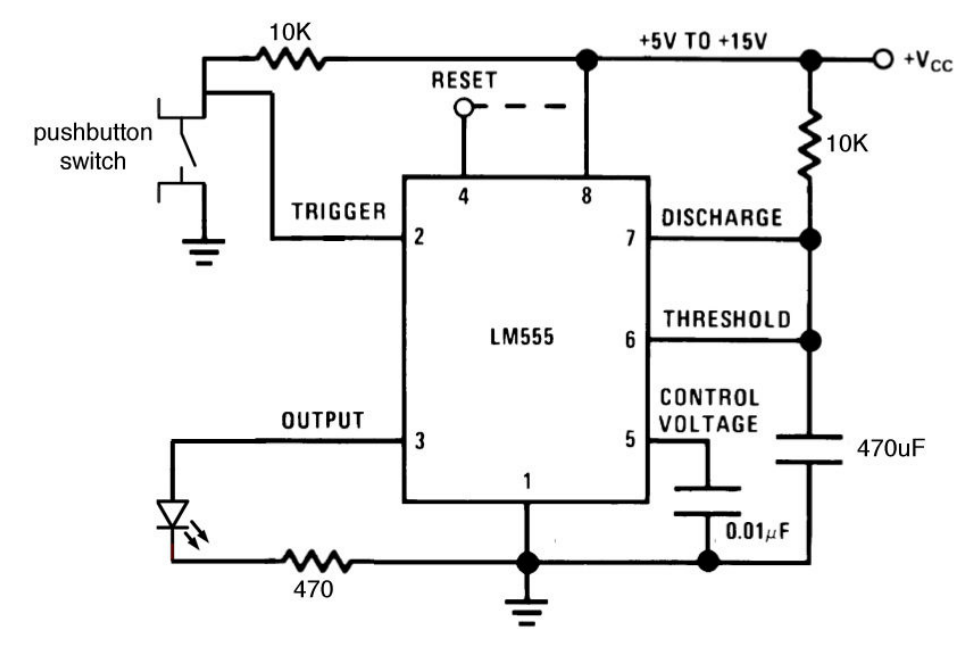
\includegraphics[width=0.75\textwidth]{DatasheetSchematic}
\centering
\caption{LM555 Example Circuit}
\end{figure}

\subsection{Setup}
KiCad is available for a wide range of operating systems. The download page is \href{http://kicad-pcb.org/download/}{\textbf{here}}. For Mac, make sure to get the ``extras'' package as well. It contains a useful set of default components and footprints.

\subsection{Overview}
KiCad differs from other electronics design software in that it is extremely modular. Each section of the design process is divided into a distinct program. The KiCad getting started guide has this fantastic flowchart which is a great guide for figuring out what button to push next at any step of the design process.

KiCad has a bad habit of not labeling any buttons. However, if you hover over any button for a few seconds, a tooltip will come up explaining what the button does. Also, in any of the editors typing `?' will bring up a list of keyboard commands.

\begin{figure}[H]
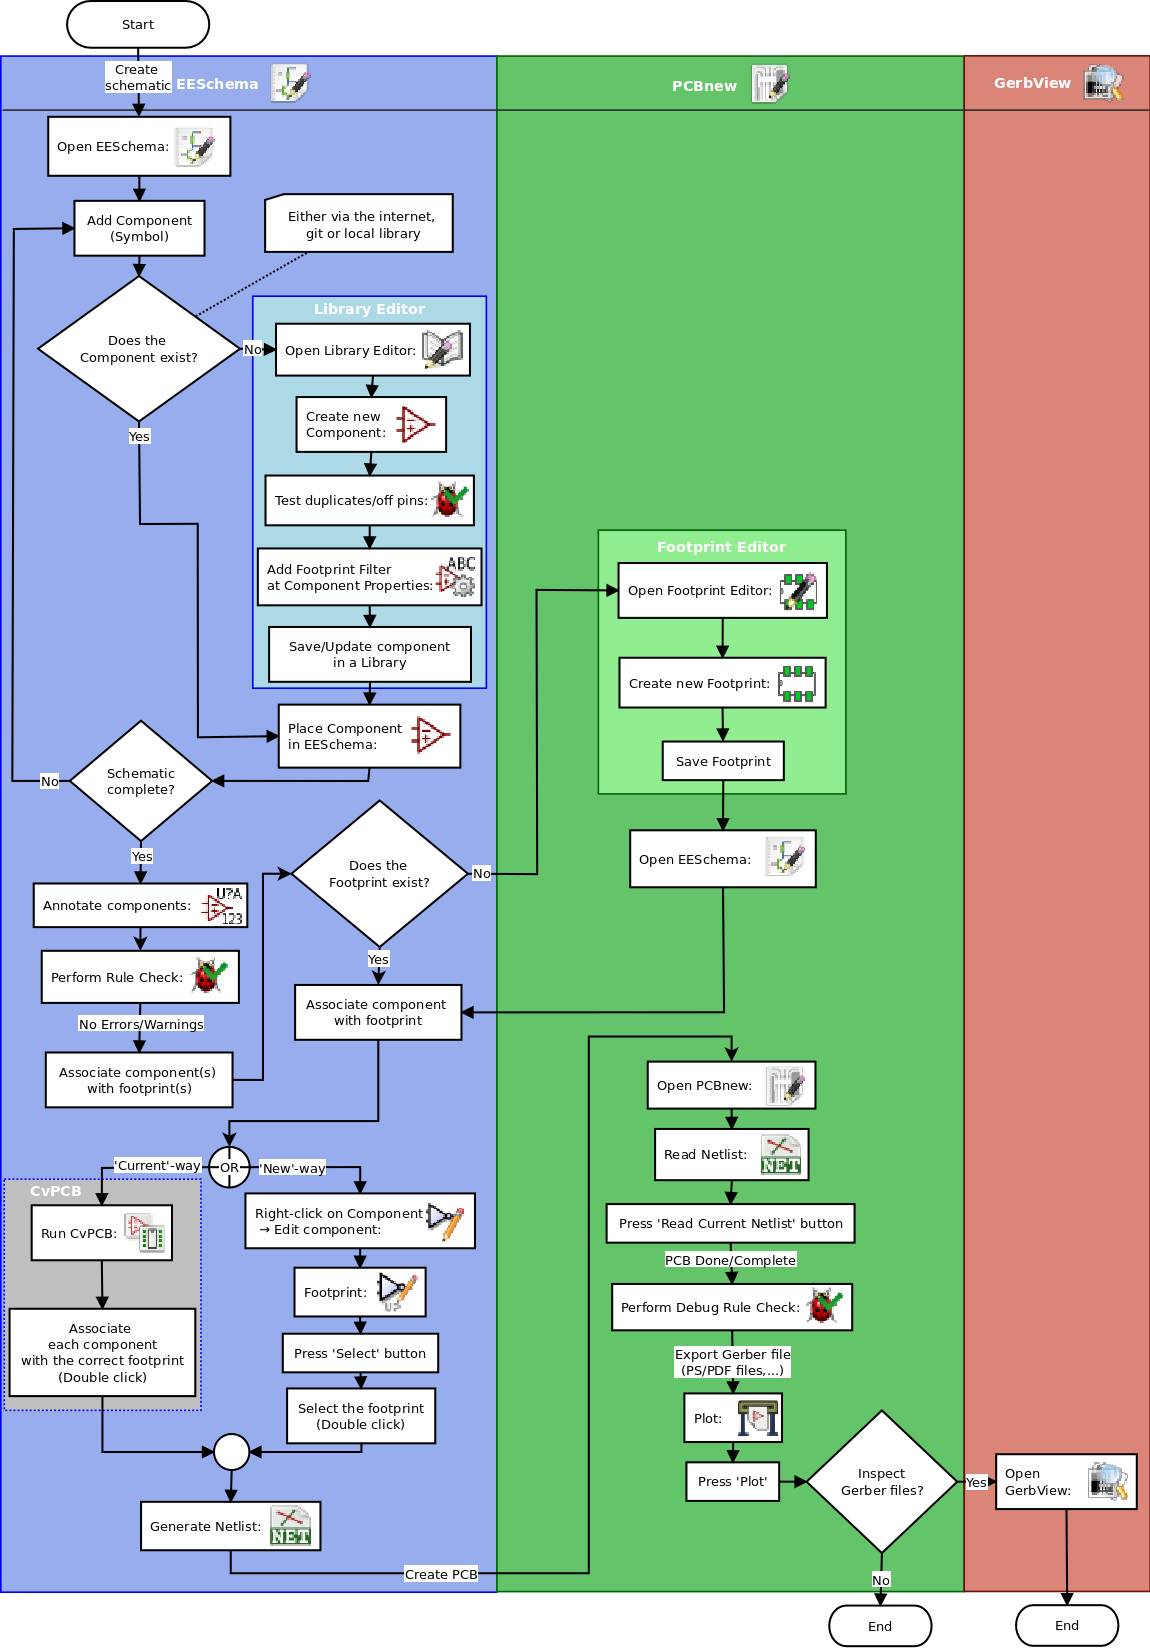
\includegraphics[width=0.9\textwidth]{kicad_flowchart}
\centering
\caption{KiCad PCB workflow flowchart}
\end{figure}

\section{Create a Project}
The first step is to create a project, which will serve as a general container for KiCad to keep track of the mess of files that will make up your design. Open up the KiCad application. Select \textbf{File $\rightarrow$ New project}, and pick a nice name and location to save the project. For this tutorial, the project name is ``LEDBlinker''. As the dialog will remind you, it is a very good idea to create a project in its own folder. 

Once this step is done, you should see a \texttt{.pro}, \texttt{.kicad\_pcb}, and \texttt{.sch} file show up in your project directory and the KiCad application's sidebar.

\begin{figure}[H]
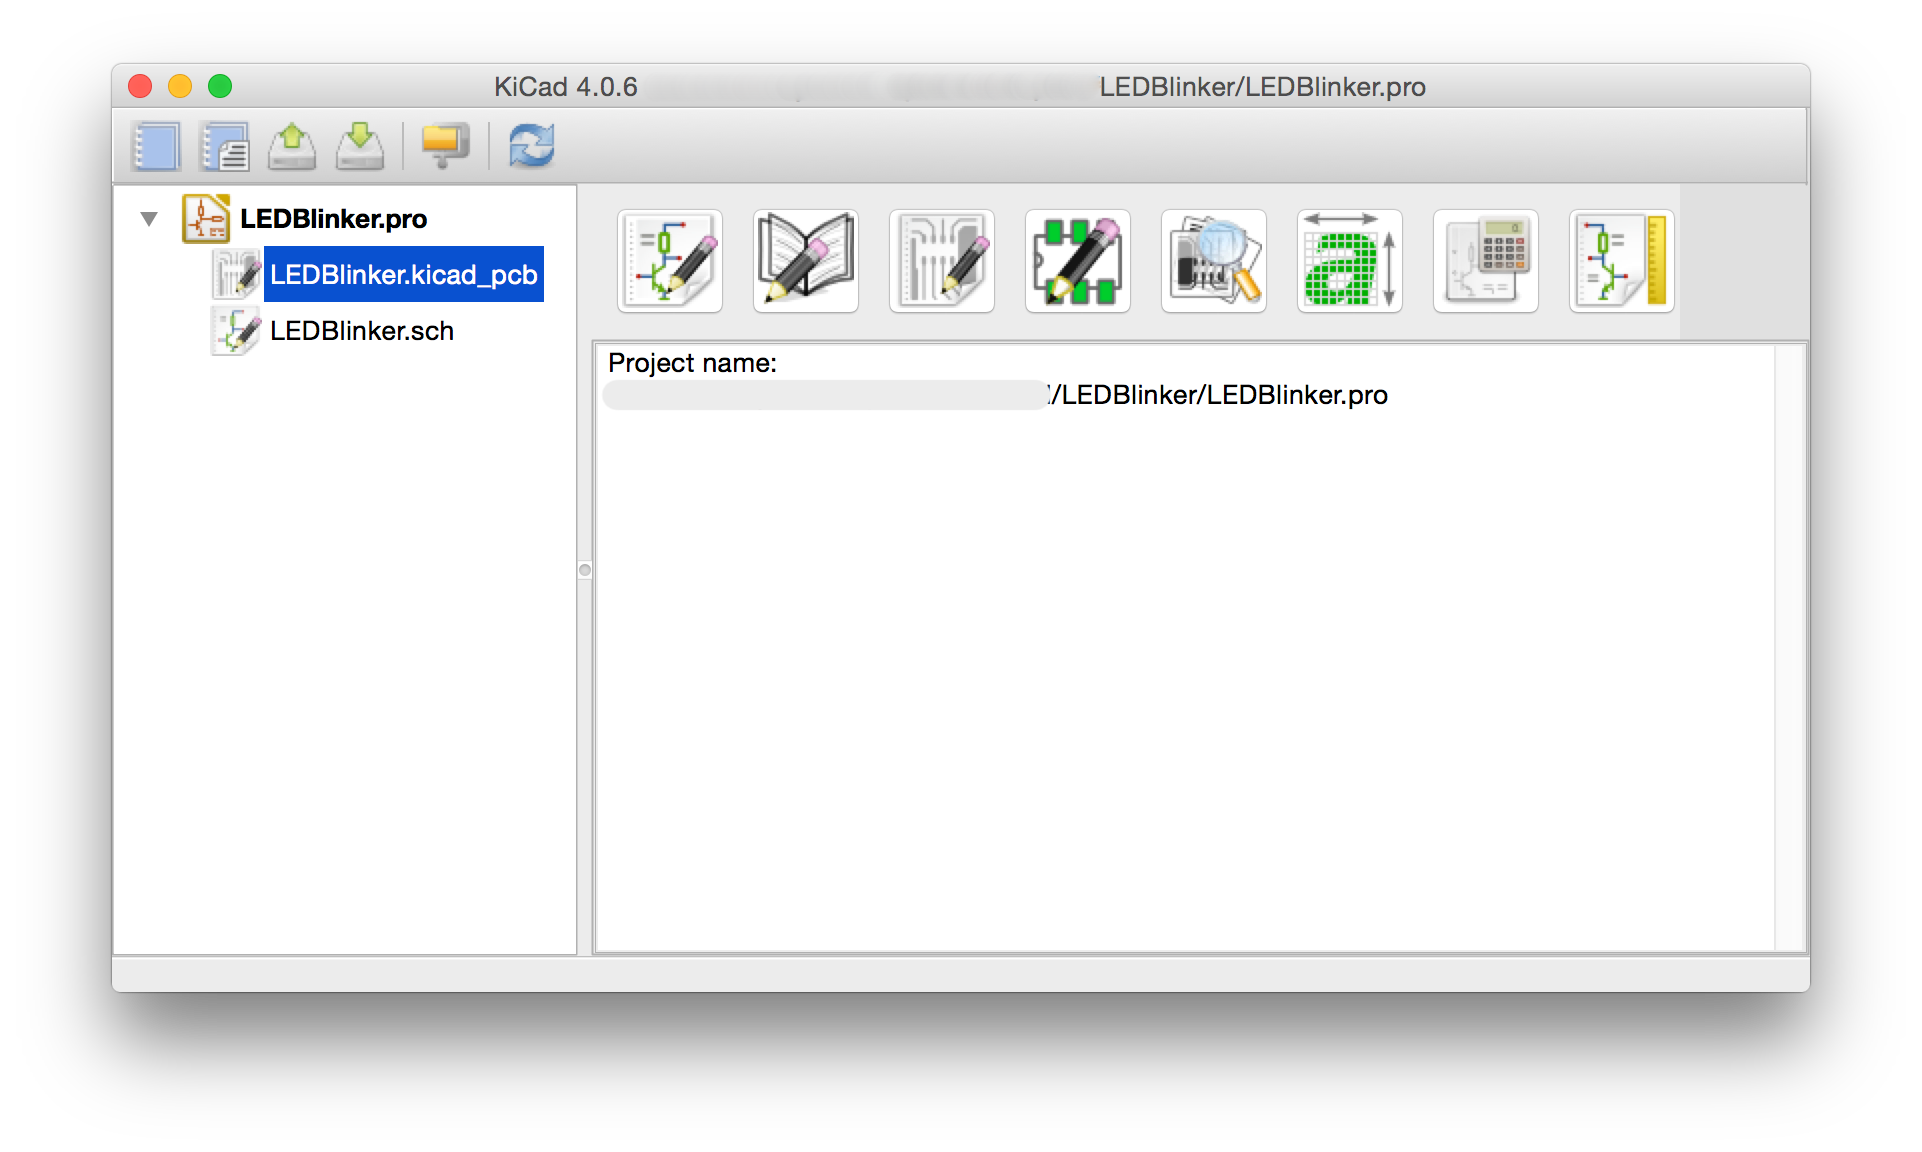
\includegraphics[width=0.75\textwidth]{CreateProject}
\centering
\caption{After project creation}
\end{figure}

From this screen, you can double click on the files to open them for editing. The large square buttons allow you to directly launch the various utilities within KiCad.

\begin{figure}[H]
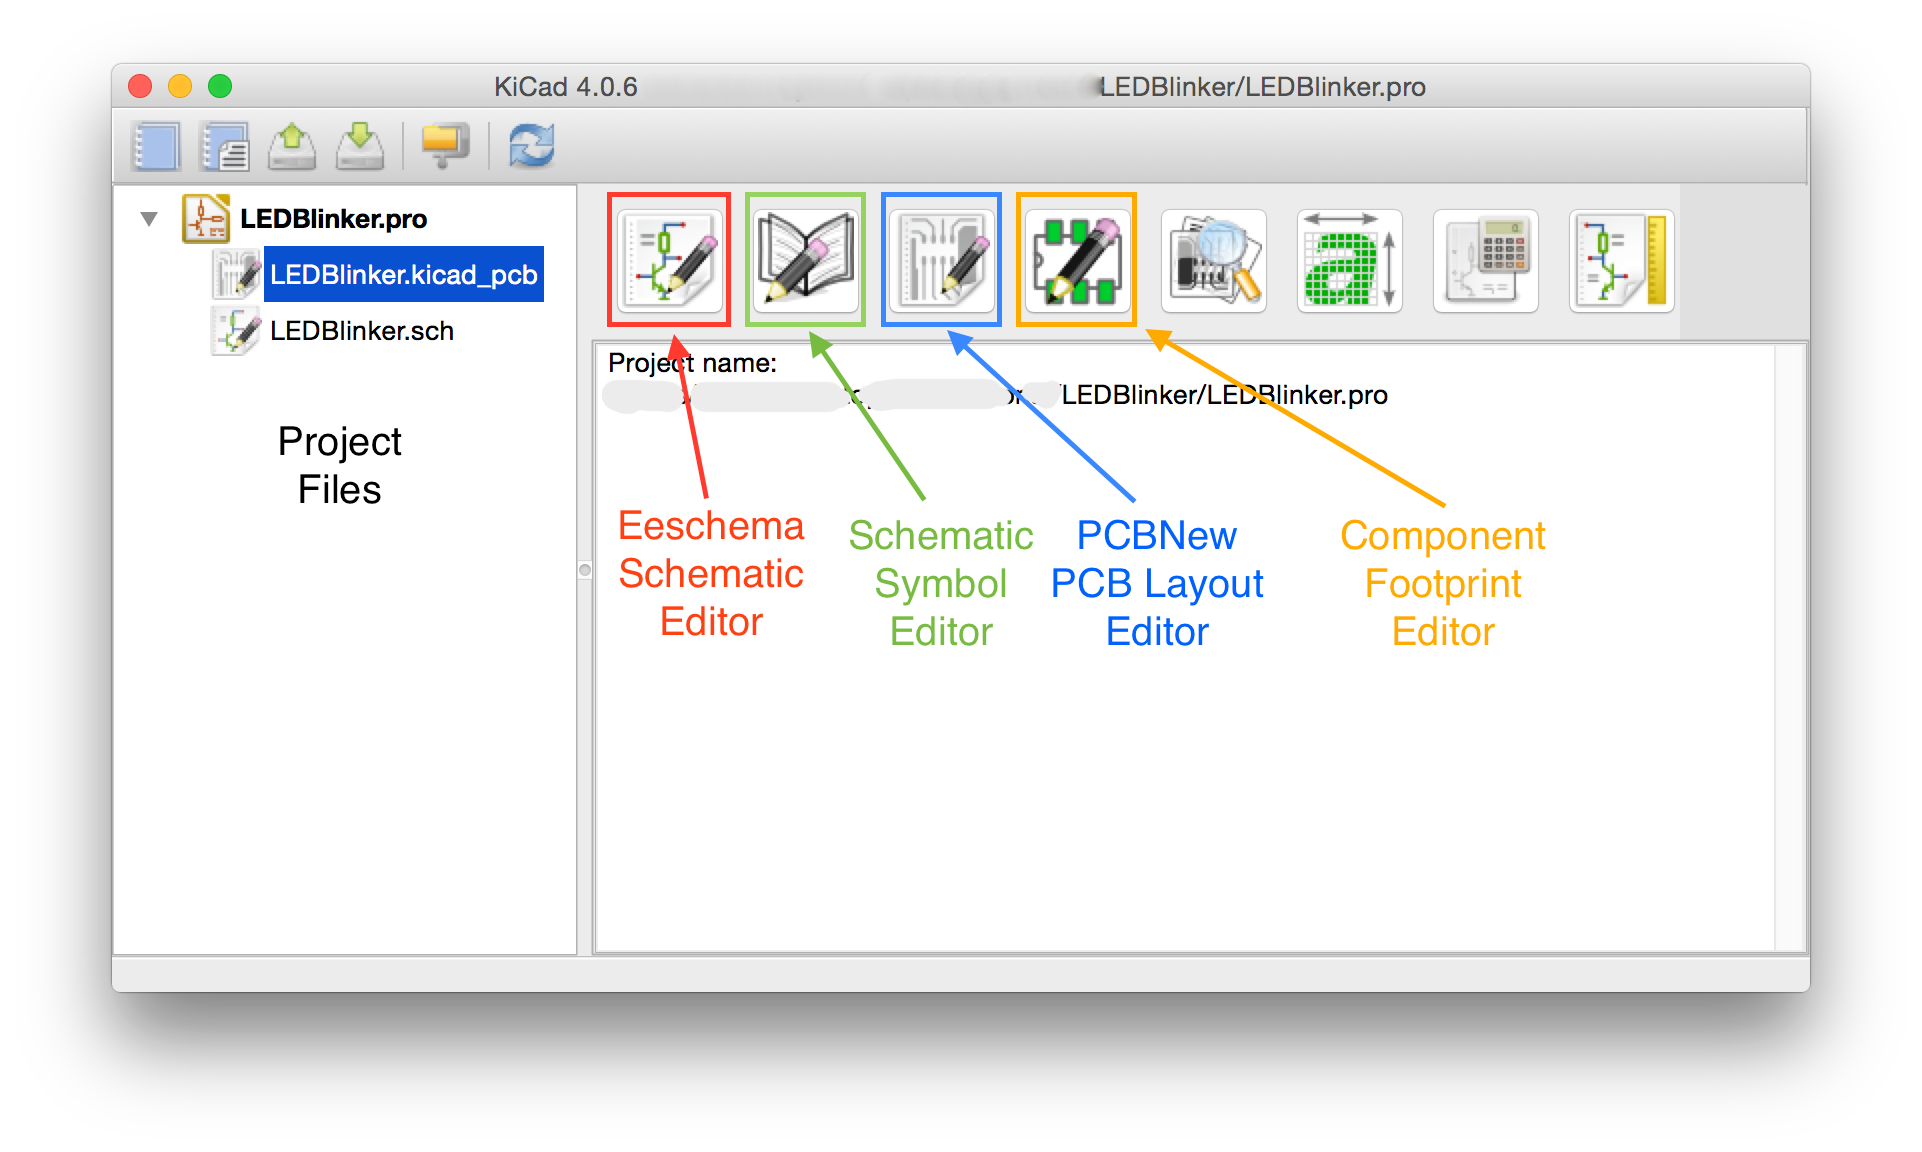
\includegraphics[width=0.75\textwidth]{CreateProject_annotated}
\centering
\caption{KiCad Main Window}
\end{figure}

\section{Schematic}
The schematic defines the components that make up the circuit and the connections between them at a high level. Double click on the schematic file in the side bar, or the schematic editor button to launch Eeschema, the schematic editor application. Once the file loads, you should be looking at a blank schematic sheet.

\begin{figure}[H]
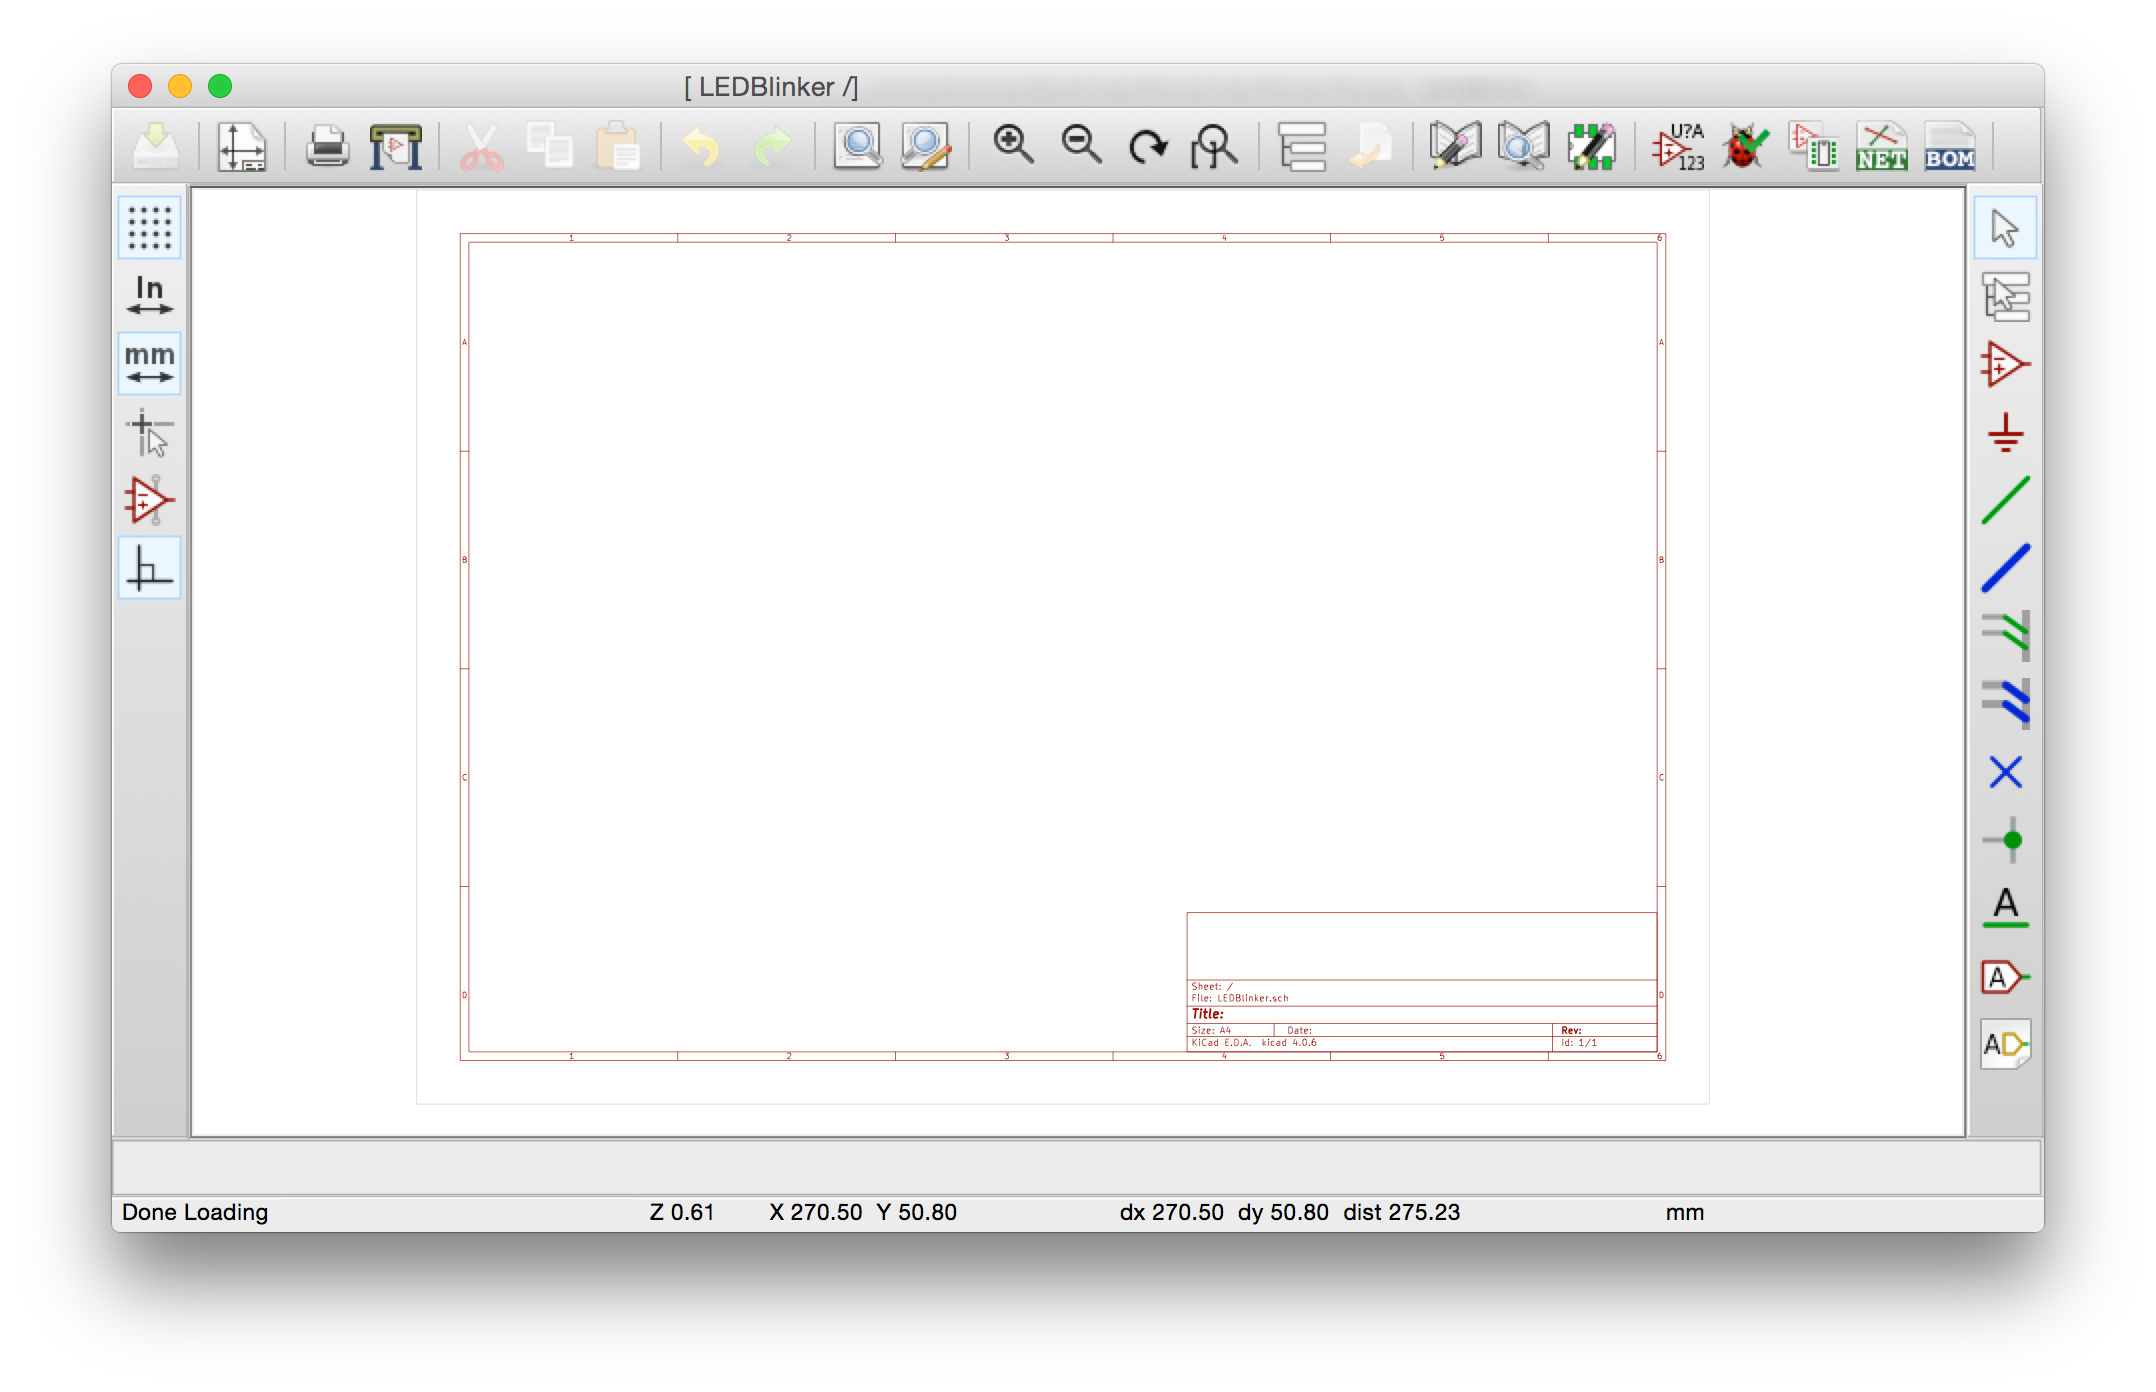
\includegraphics[width=0.75\textwidth]{BlankSchematic}
\centering
\caption{Blank Schematic}
\end{figure}

\subsection{Page Settings}
Just as in high school, you should always put your name on your work. So, the first thing to do is to adjust your page settings under \textbf{File $\rightarrow$ Page Settings}. Here are some options you should set for every design you make:
\begin{itemize}
	\item Page size and orientation (left sidebar)
	\item Date
	\item Revision number
	\item Title
	\item Company (Good place to put your name if this is a personal project)
	\item Comment 1 (Put your name here if the Company field is filled)
\end{itemize}

\begin{figure}[H]
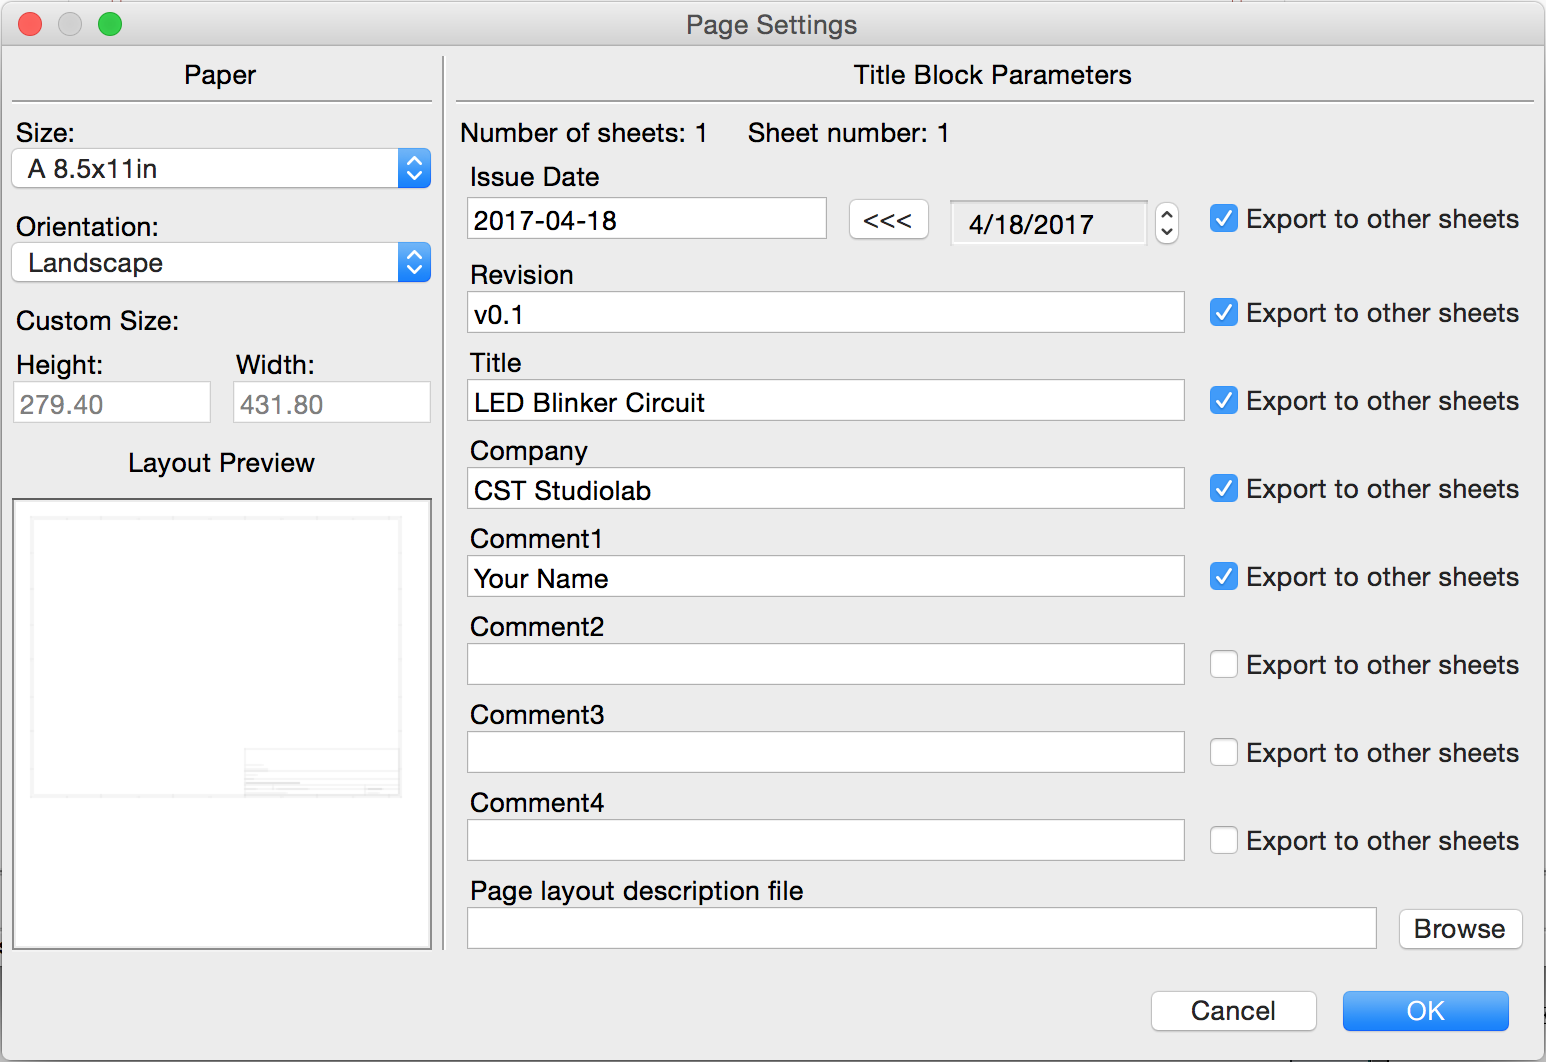
\includegraphics[width=0.75\textwidth]{PageSettings}
\centering
\caption{Schematic Page Settings}
\end{figure}

Checking the \textbf{``Export to Other Sheets''} option will copy these settings to other schematic documents in your project. Click OK to save your settings, and you should see the title block of the schematic update with the information you entered.

\subsection{Moving Around}
Now that the page is set up, we can start the business of drawing our schematic. To move around, use the scroll wheel on your mouse to zoom in. Holding the 3rd mouse button and dragging pans the canvas. To practice, zoom in on the title block and make sure all the options you set in the last section appeared correctly.

\subsubsection{Important note for laptop users}

If you are using the trackpad on a Mac, open up the the main preferences (\textbf{KiCad $\rightarrow$ Preferences}) and check the option to \textbf{``Use Touchpad to Pan''}. This will enable touchpad support so that you can scroll and zoom with the trackpad just like any other application.  If you're using an external mouse, leave this option unchecked.

\begin{figure}[H]
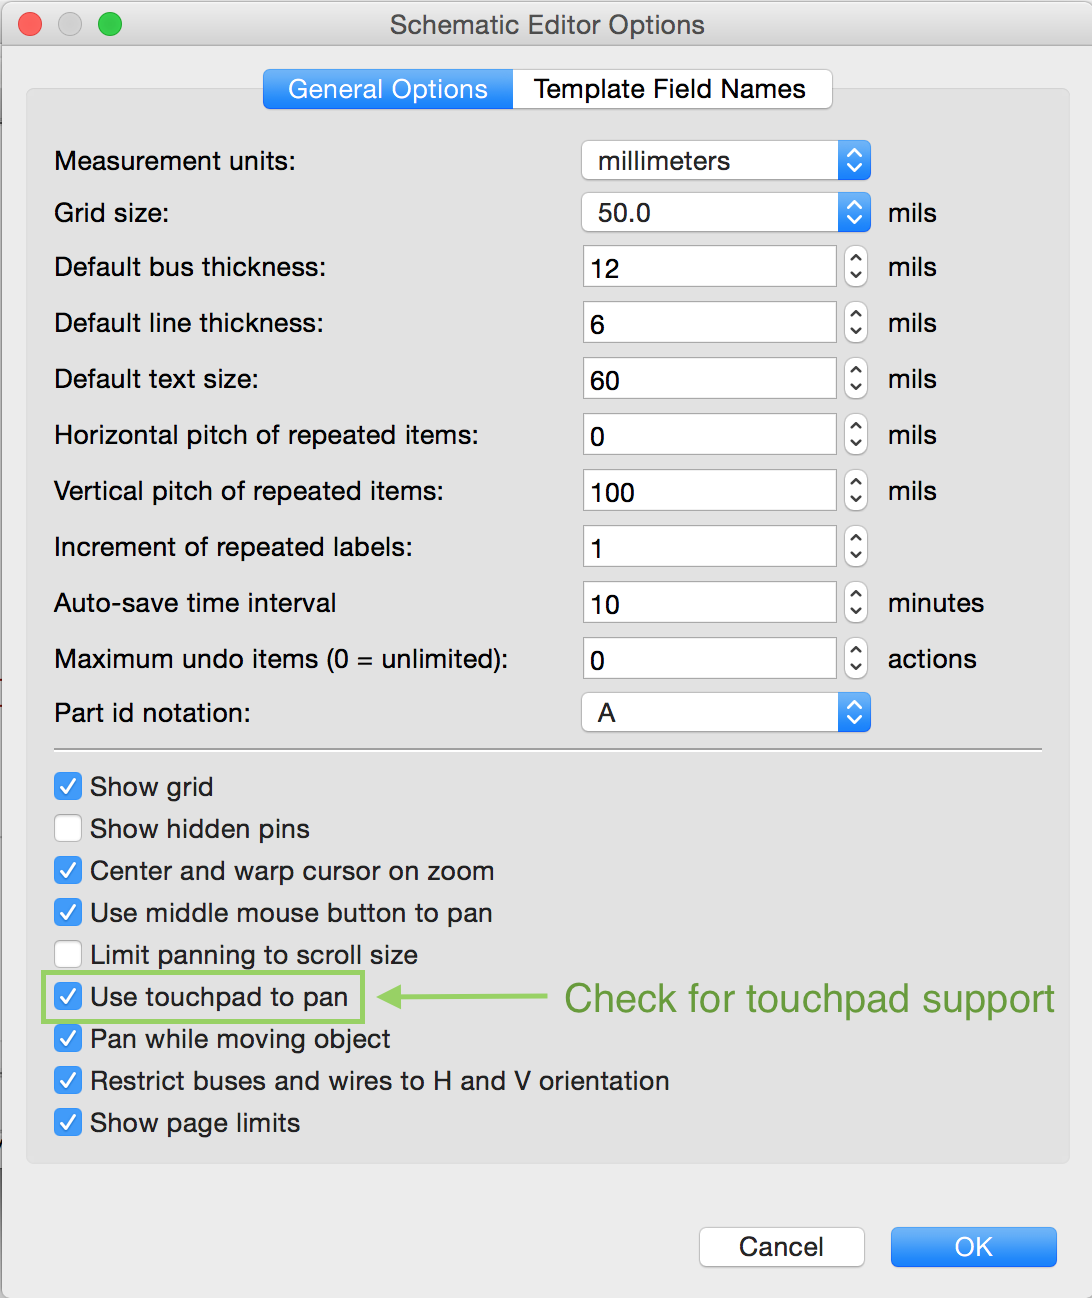
\includegraphics[width=0.5\textwidth]{TouchpadPan}
\centering
\caption{Touchpad Pan Option}
\end{figure}

\subsection{Add Components}
Let's add in the components of this circuit. Switch to the add component tool by clicking on the Add Component button on the right toolbar or pressing the \textbf{`A'} key. Click somewhere on the canvas to place a component.
\begin{figure}[H]

\includegraphics{AddComponent}
\centering
\caption{Add Component Tool Button}
\end{figure}

A dialog box will pop up asking you which component to place.
\begin{figure}[H]
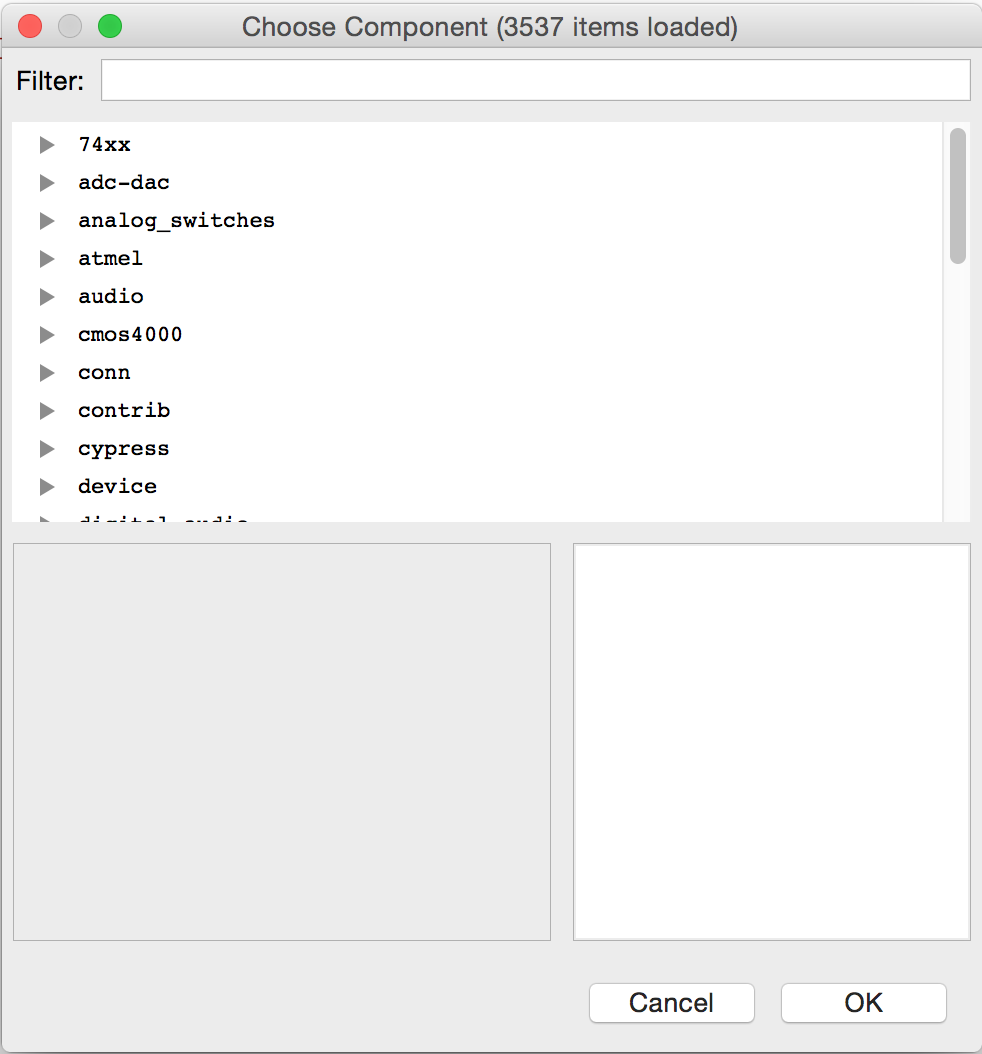
\includegraphics[width=0.75\textwidth]{AddComponentDialog}
\centering
\caption{Add Component Dialog}
\end{figure}

You can search for specific components using the top dialog box. Let's find the LM555 timer chip at the center of the circuit. Type `555' into the search box and select the LM555 component.

\begin{figure}[H]
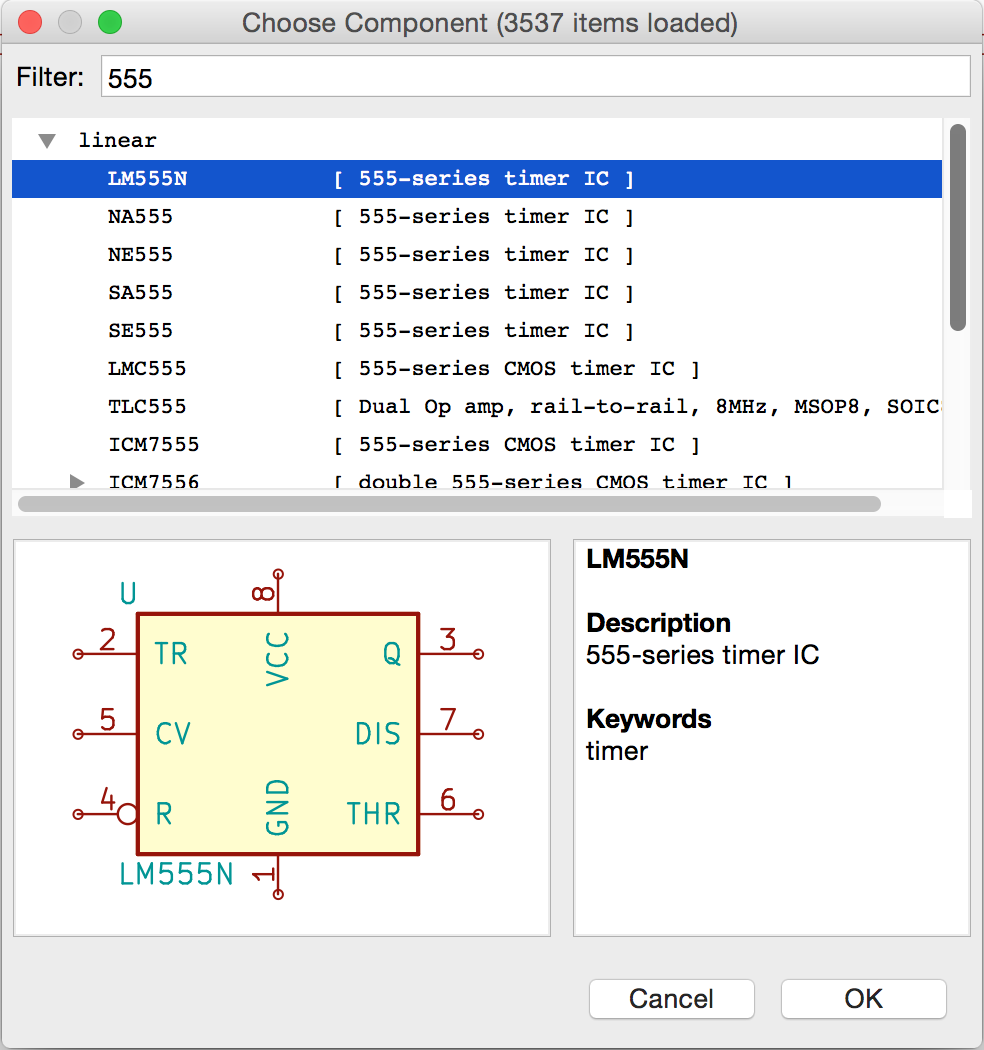
\includegraphics[width=0.75\textwidth]{AddLM555}
\centering
\caption{Add LM555}
\end{figure}

Click OK on the dialog to select the LM555. You should see a ghost of the component following your cursor. Click to place the LM555 in the center of your schematic.

\begin{figure}[H]
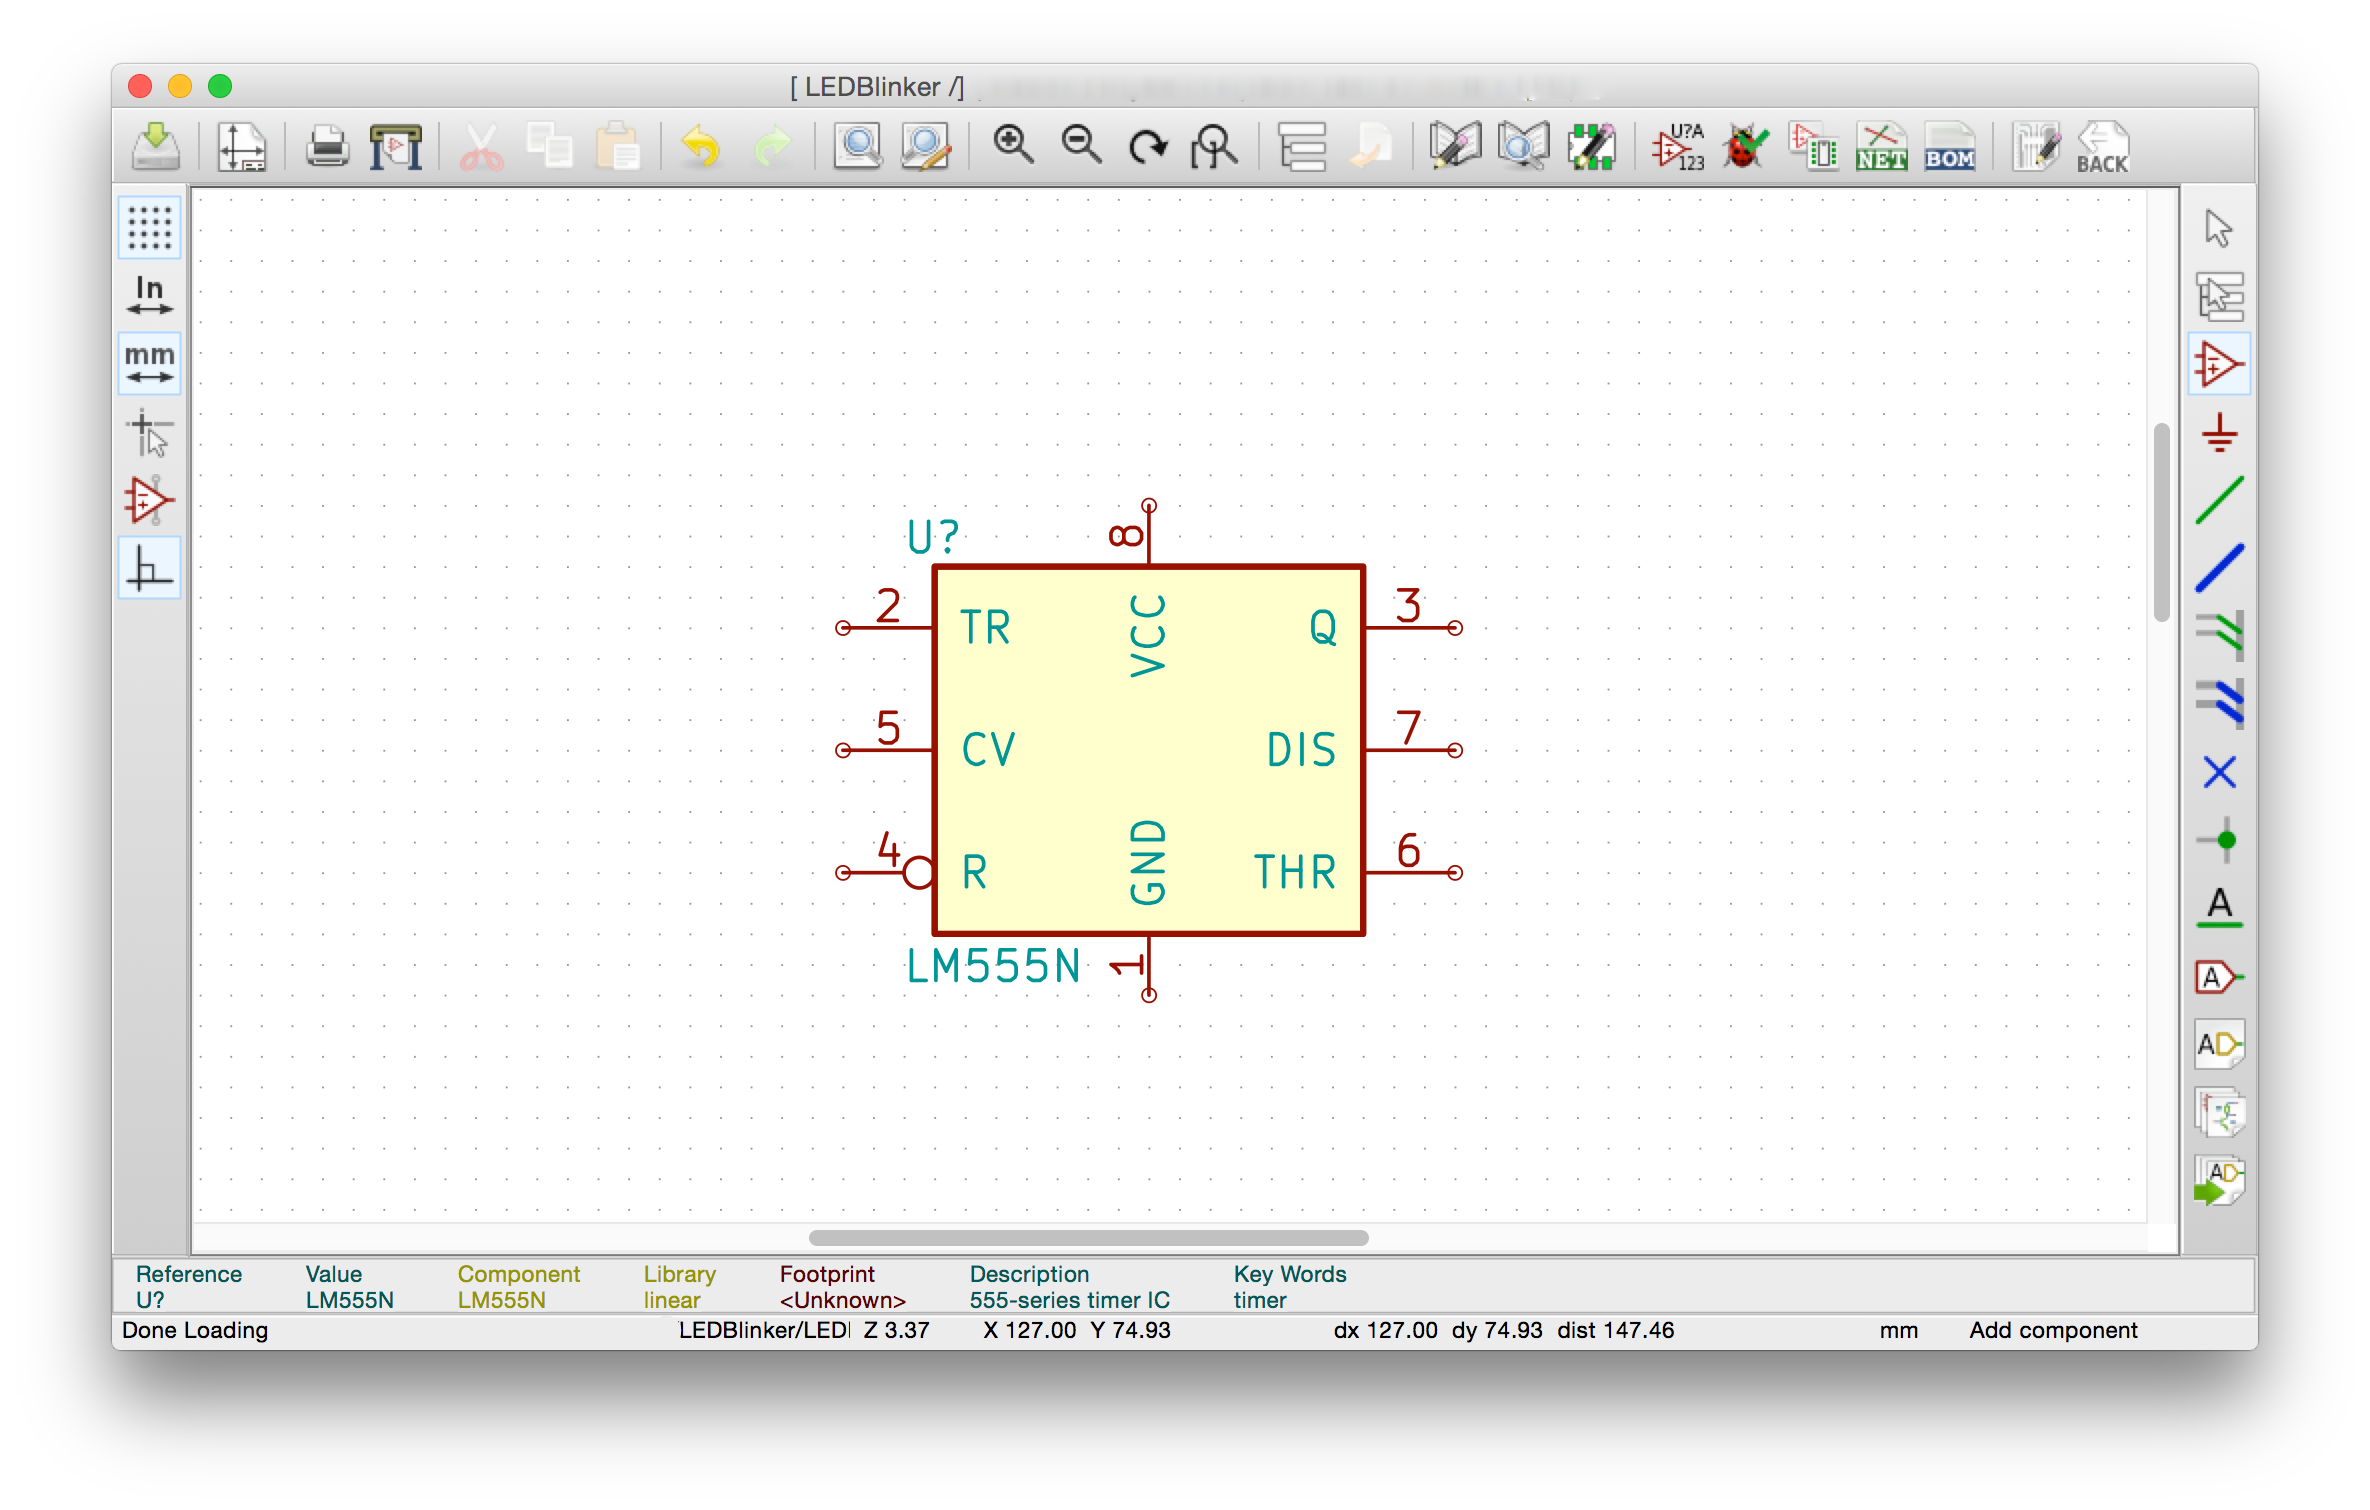
\includegraphics[width=0.75\textwidth]{PlacedLM555}
\centering
\caption{Placed LM555}
\end{figure}

If you click again, the select component dialog will reappear for selecting the next component to place. Try searching for and placing the rest of the components in the circuit. You'll need 3 resistors, 2 capacitors, and a LED. The Don't worry about exactly matching the same layout as in the example circuit diagram, we'll be reorganizing the components later.

\begin{figure}[H]
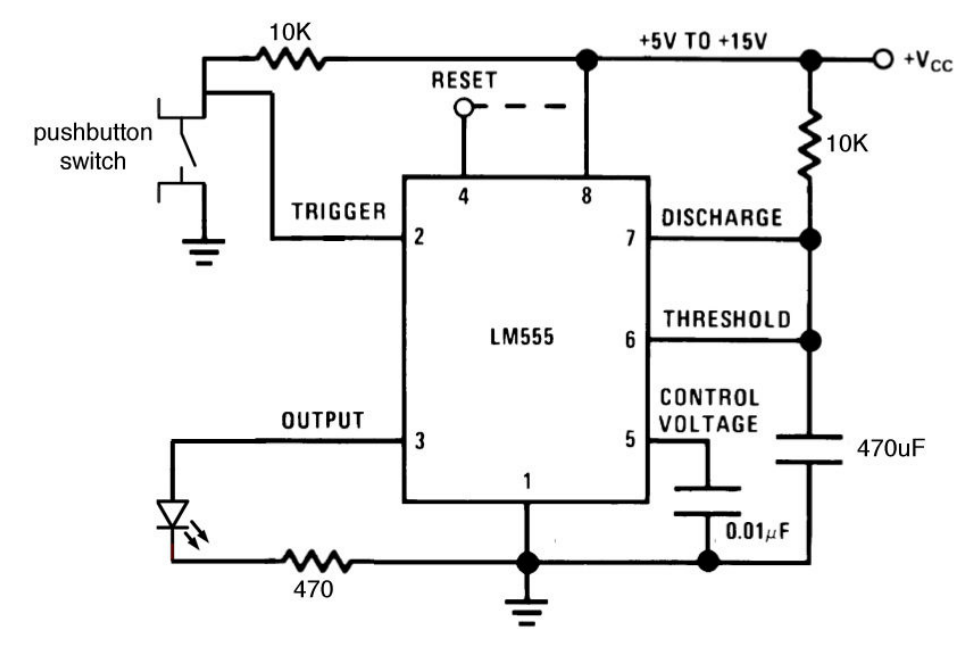
\includegraphics[width=0.75\textwidth]{DatasheetSchematic}
\centering
\caption{LM555 Example Circuit}
\end{figure}

Once you've finished adding the components, your canvas should look something like this:

\begin{figure}[H]
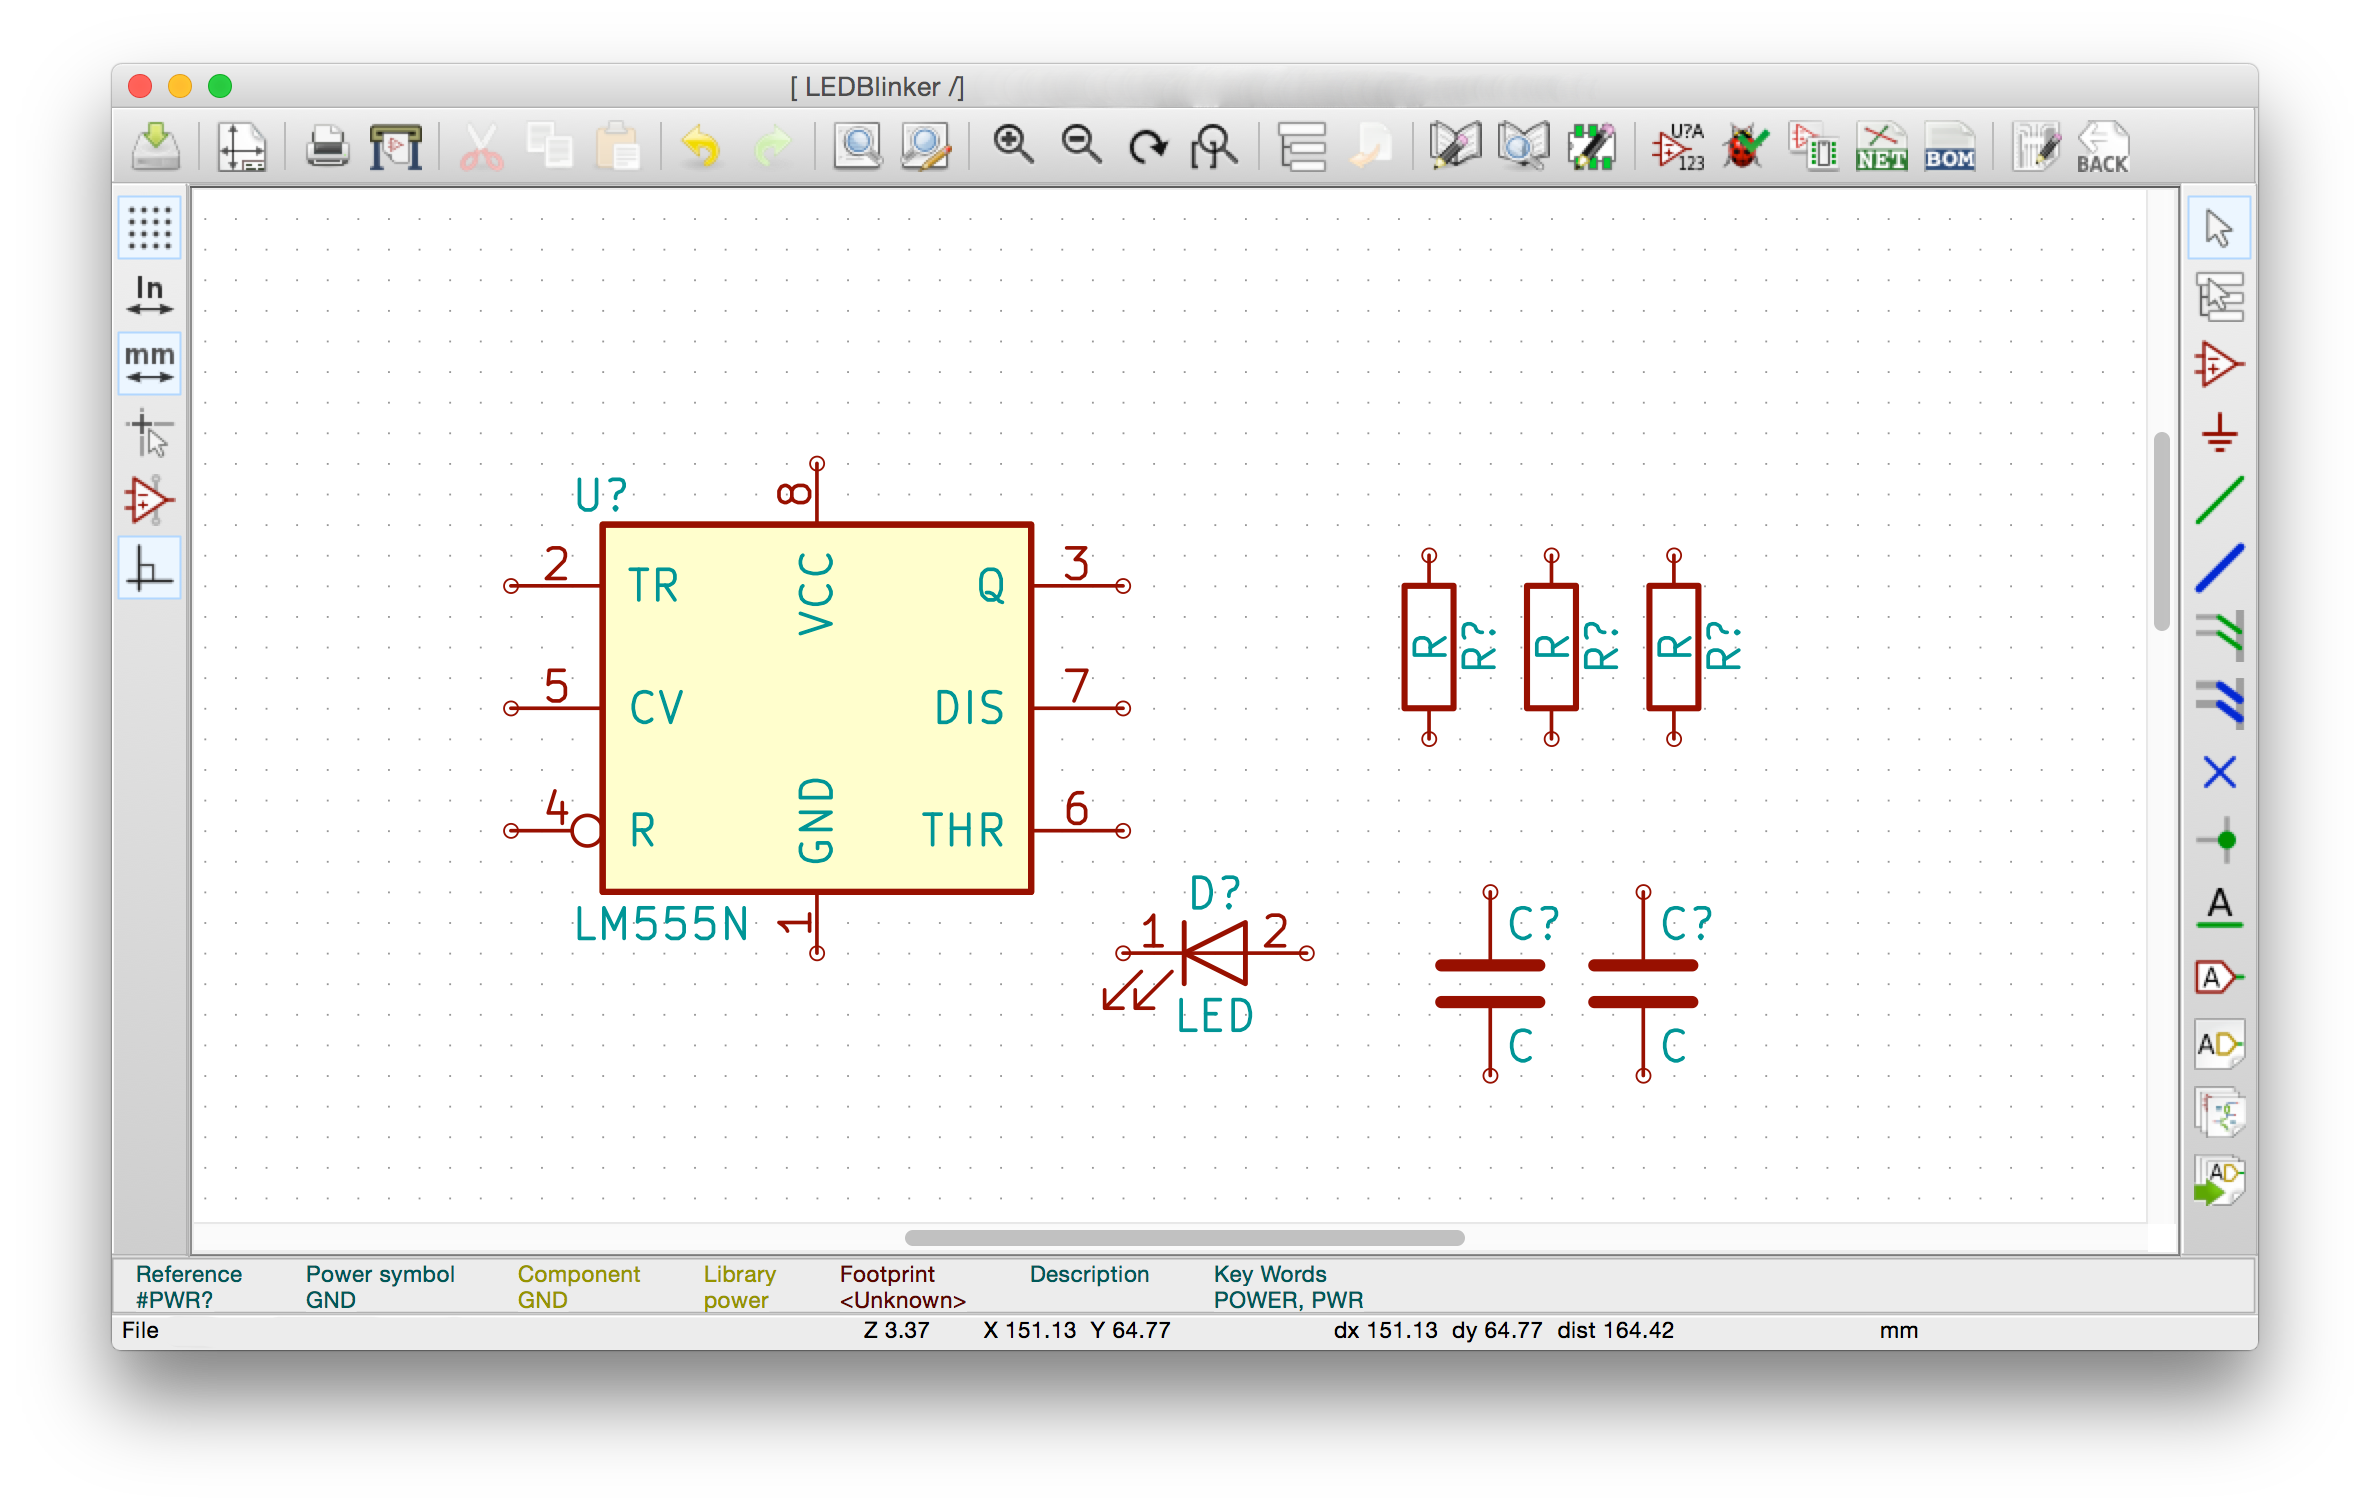
\includegraphics[width=0.75\textwidth]{AddedComponents}
\centering
\caption{All Components Added}
\end{figure}

Remember to save your work, hit \textbf{Ctrl-S} or \textbf{Cmd-S} on Mac.

\subsection{Power Ports}
Let us also place labels for the power and ground connections for this circuit. Select the power ports tool by clicking on the button that looks like a miniature ground symbol.

\begin{figure}[H]

\includegraphics{PowerSymbol}
\centering
\caption{Add Power Port Dialog}
\end{figure}

This tool acts in a similar fashion to the add component tool. Click to open the dialog to select symbols, search for a symbol, then hit OK and click to place your selected symbol. Add a VCC symbol and a GND symbol to your schematic.

\begin{figure}[H]
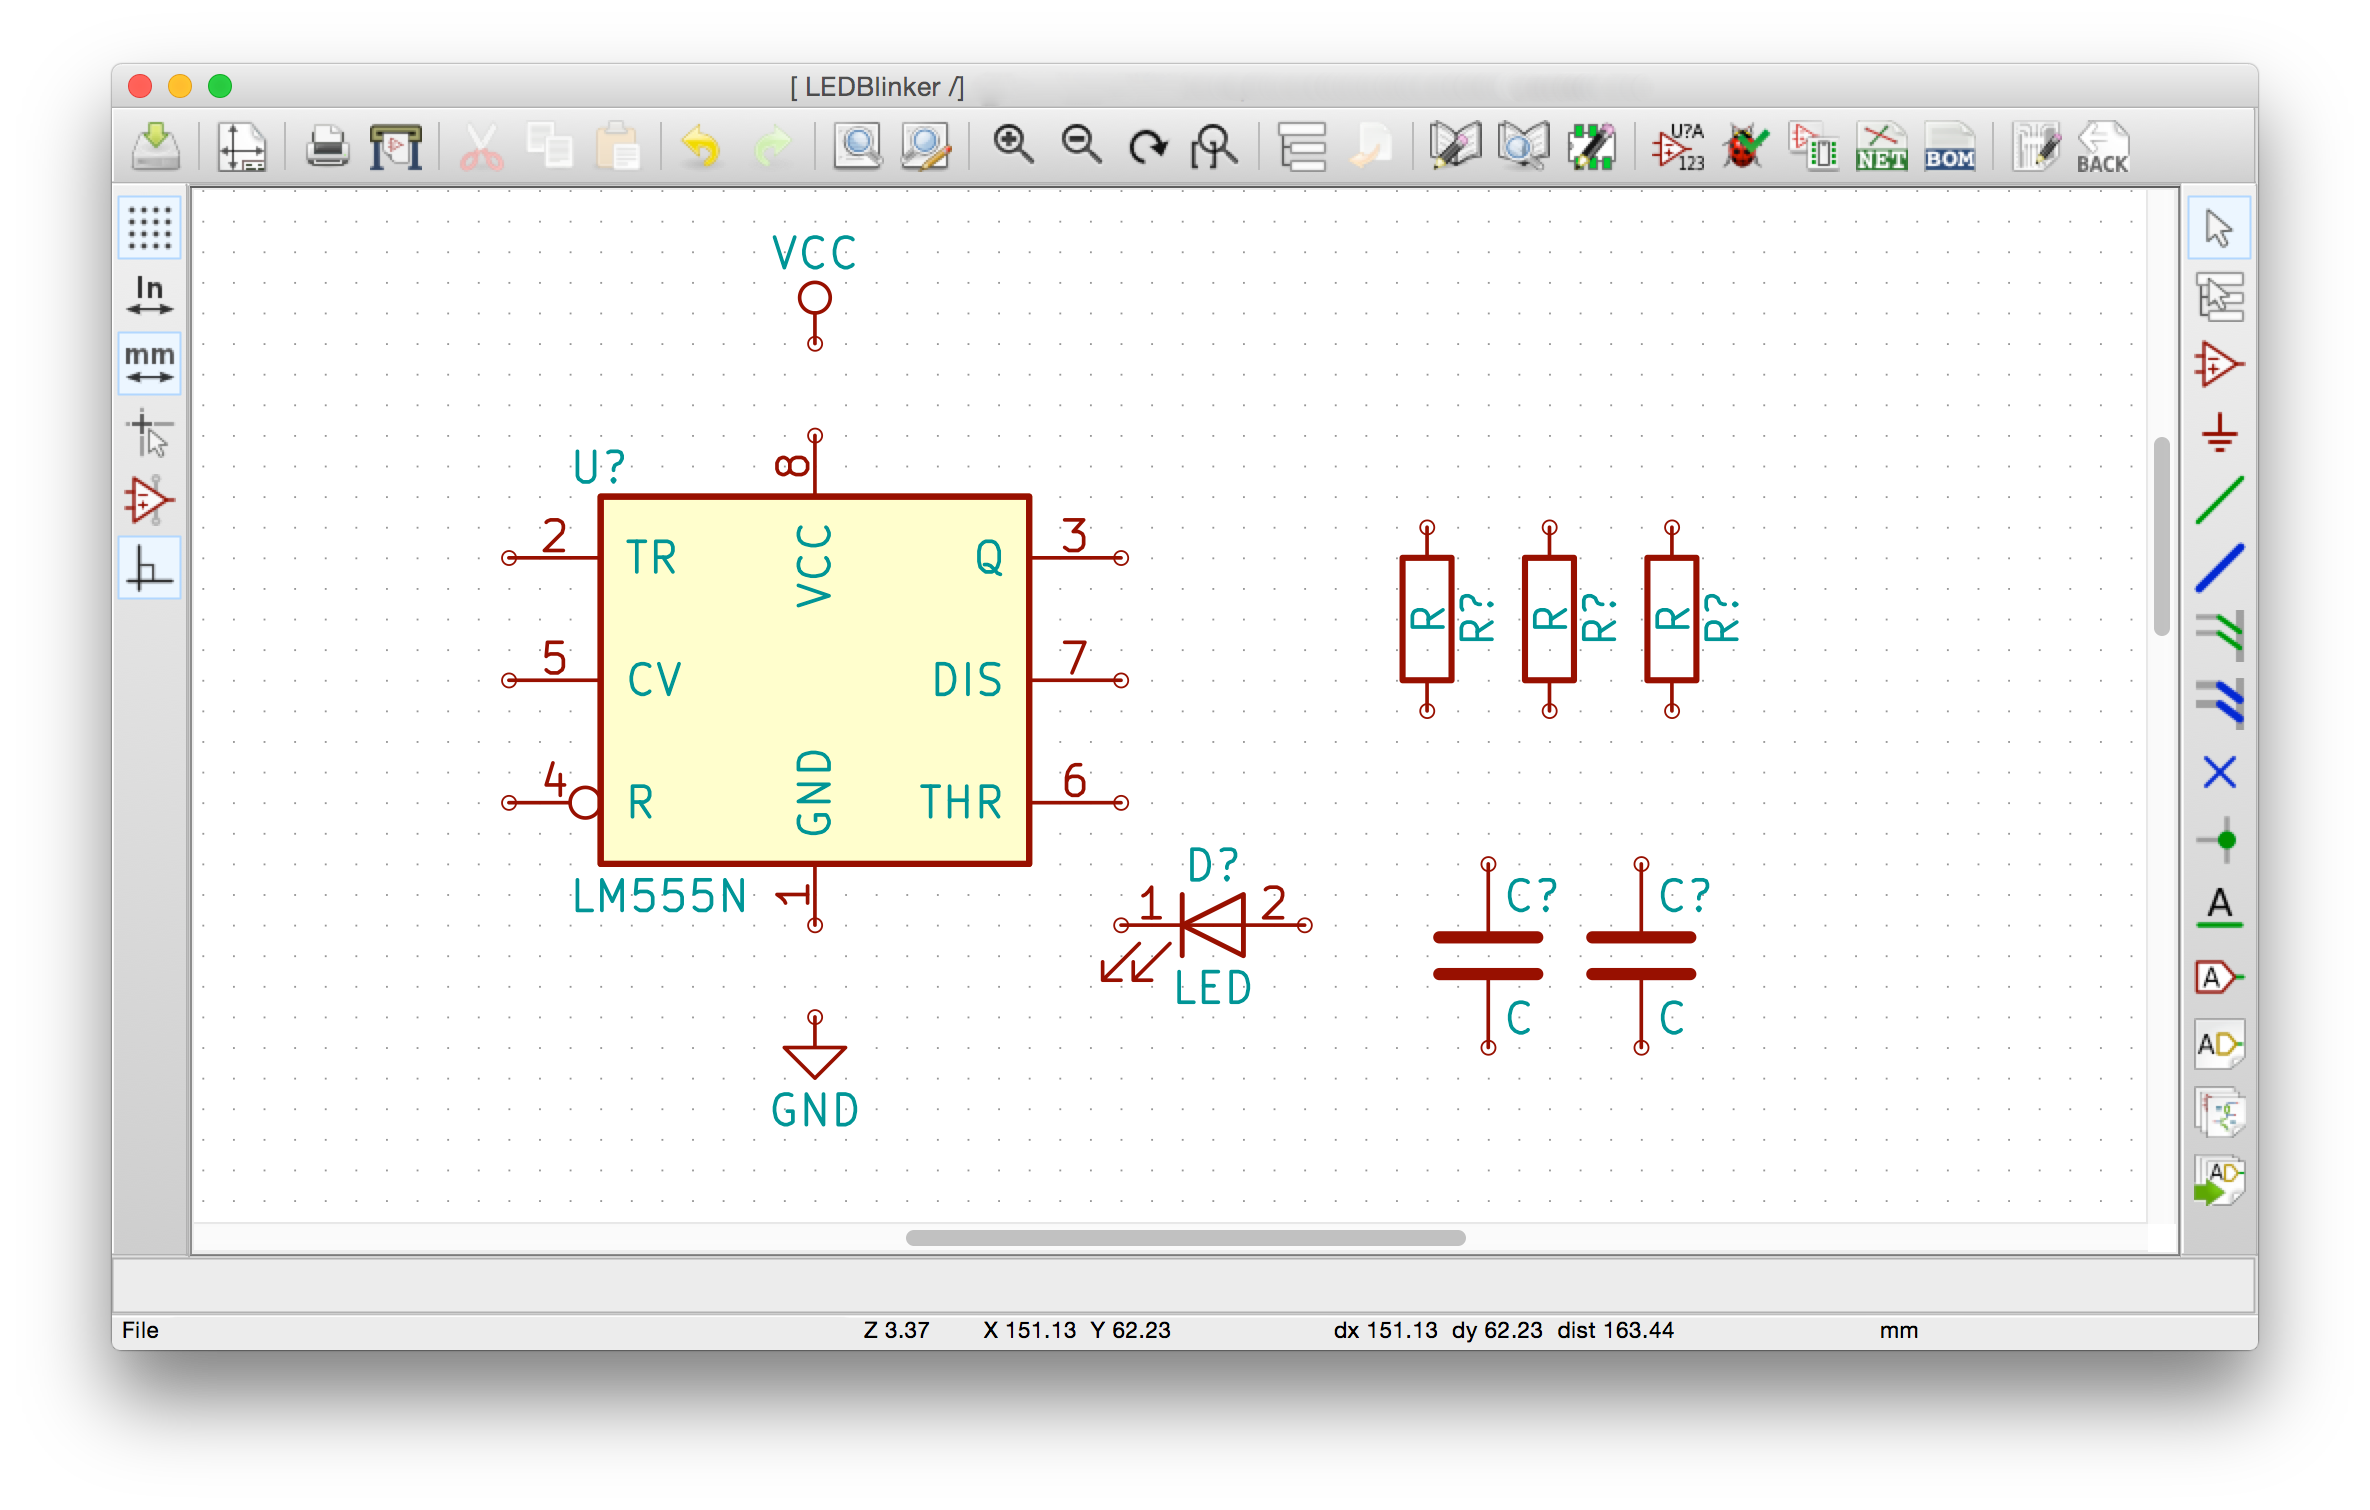
\includegraphics[width=0.75\textwidth]{AddedPowerSymbols}
\centering
\caption{Power Symbols Added}
\end{figure}

\subsection{Rearranging Components}
KiCad tends to very heavily emphasize using keyboard shortcuts. In general, you will work with one hand on the keyboard and one hand on the mouse. What is different from most other programs is that when you press a shortcut to perform an action, that action will act on whatever is underneath your cursor at that moment. Explicitly selecting objects is optional.

To demonstrate this, lets try moving the LED over to the output pin (pin 3 on the LM555). The default shortcut for moving is `\textbf{M}', so hover over the LED with your cursor and press \textbf{M}. The LED will start following your cursor around the canvas. Click to place the LED down again.

Let's rotate the LED. The hotkey for rotation is `\textbf{R}', so hover over the LED and press \textbf{R} until it is facing down.

If there are multiple objects under the cursor, a small dialog will appear to clarify which object you actually want to work with. This often happens if there are labels or pieces of text overlapping a component. Simply select the correct object in the dialog to continue.

If you want to manipulate multiple objects at once, click and drag to create a selection box. When you release the mouse, anything touching the selection box will be moved. Right click to show other operations, which will be applied to the entire group.

\begin{figure}[H]
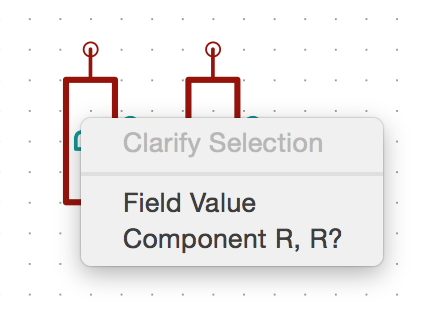
\includegraphics{ClarifySelection}
\centering
\caption{Clarify Selection Dialog}
\end{figure}

Rearrange the components around the LM555 so that they are roughly near the pins they need to be connected to. For reference, here is an example layout:

\begin{figure}[H]
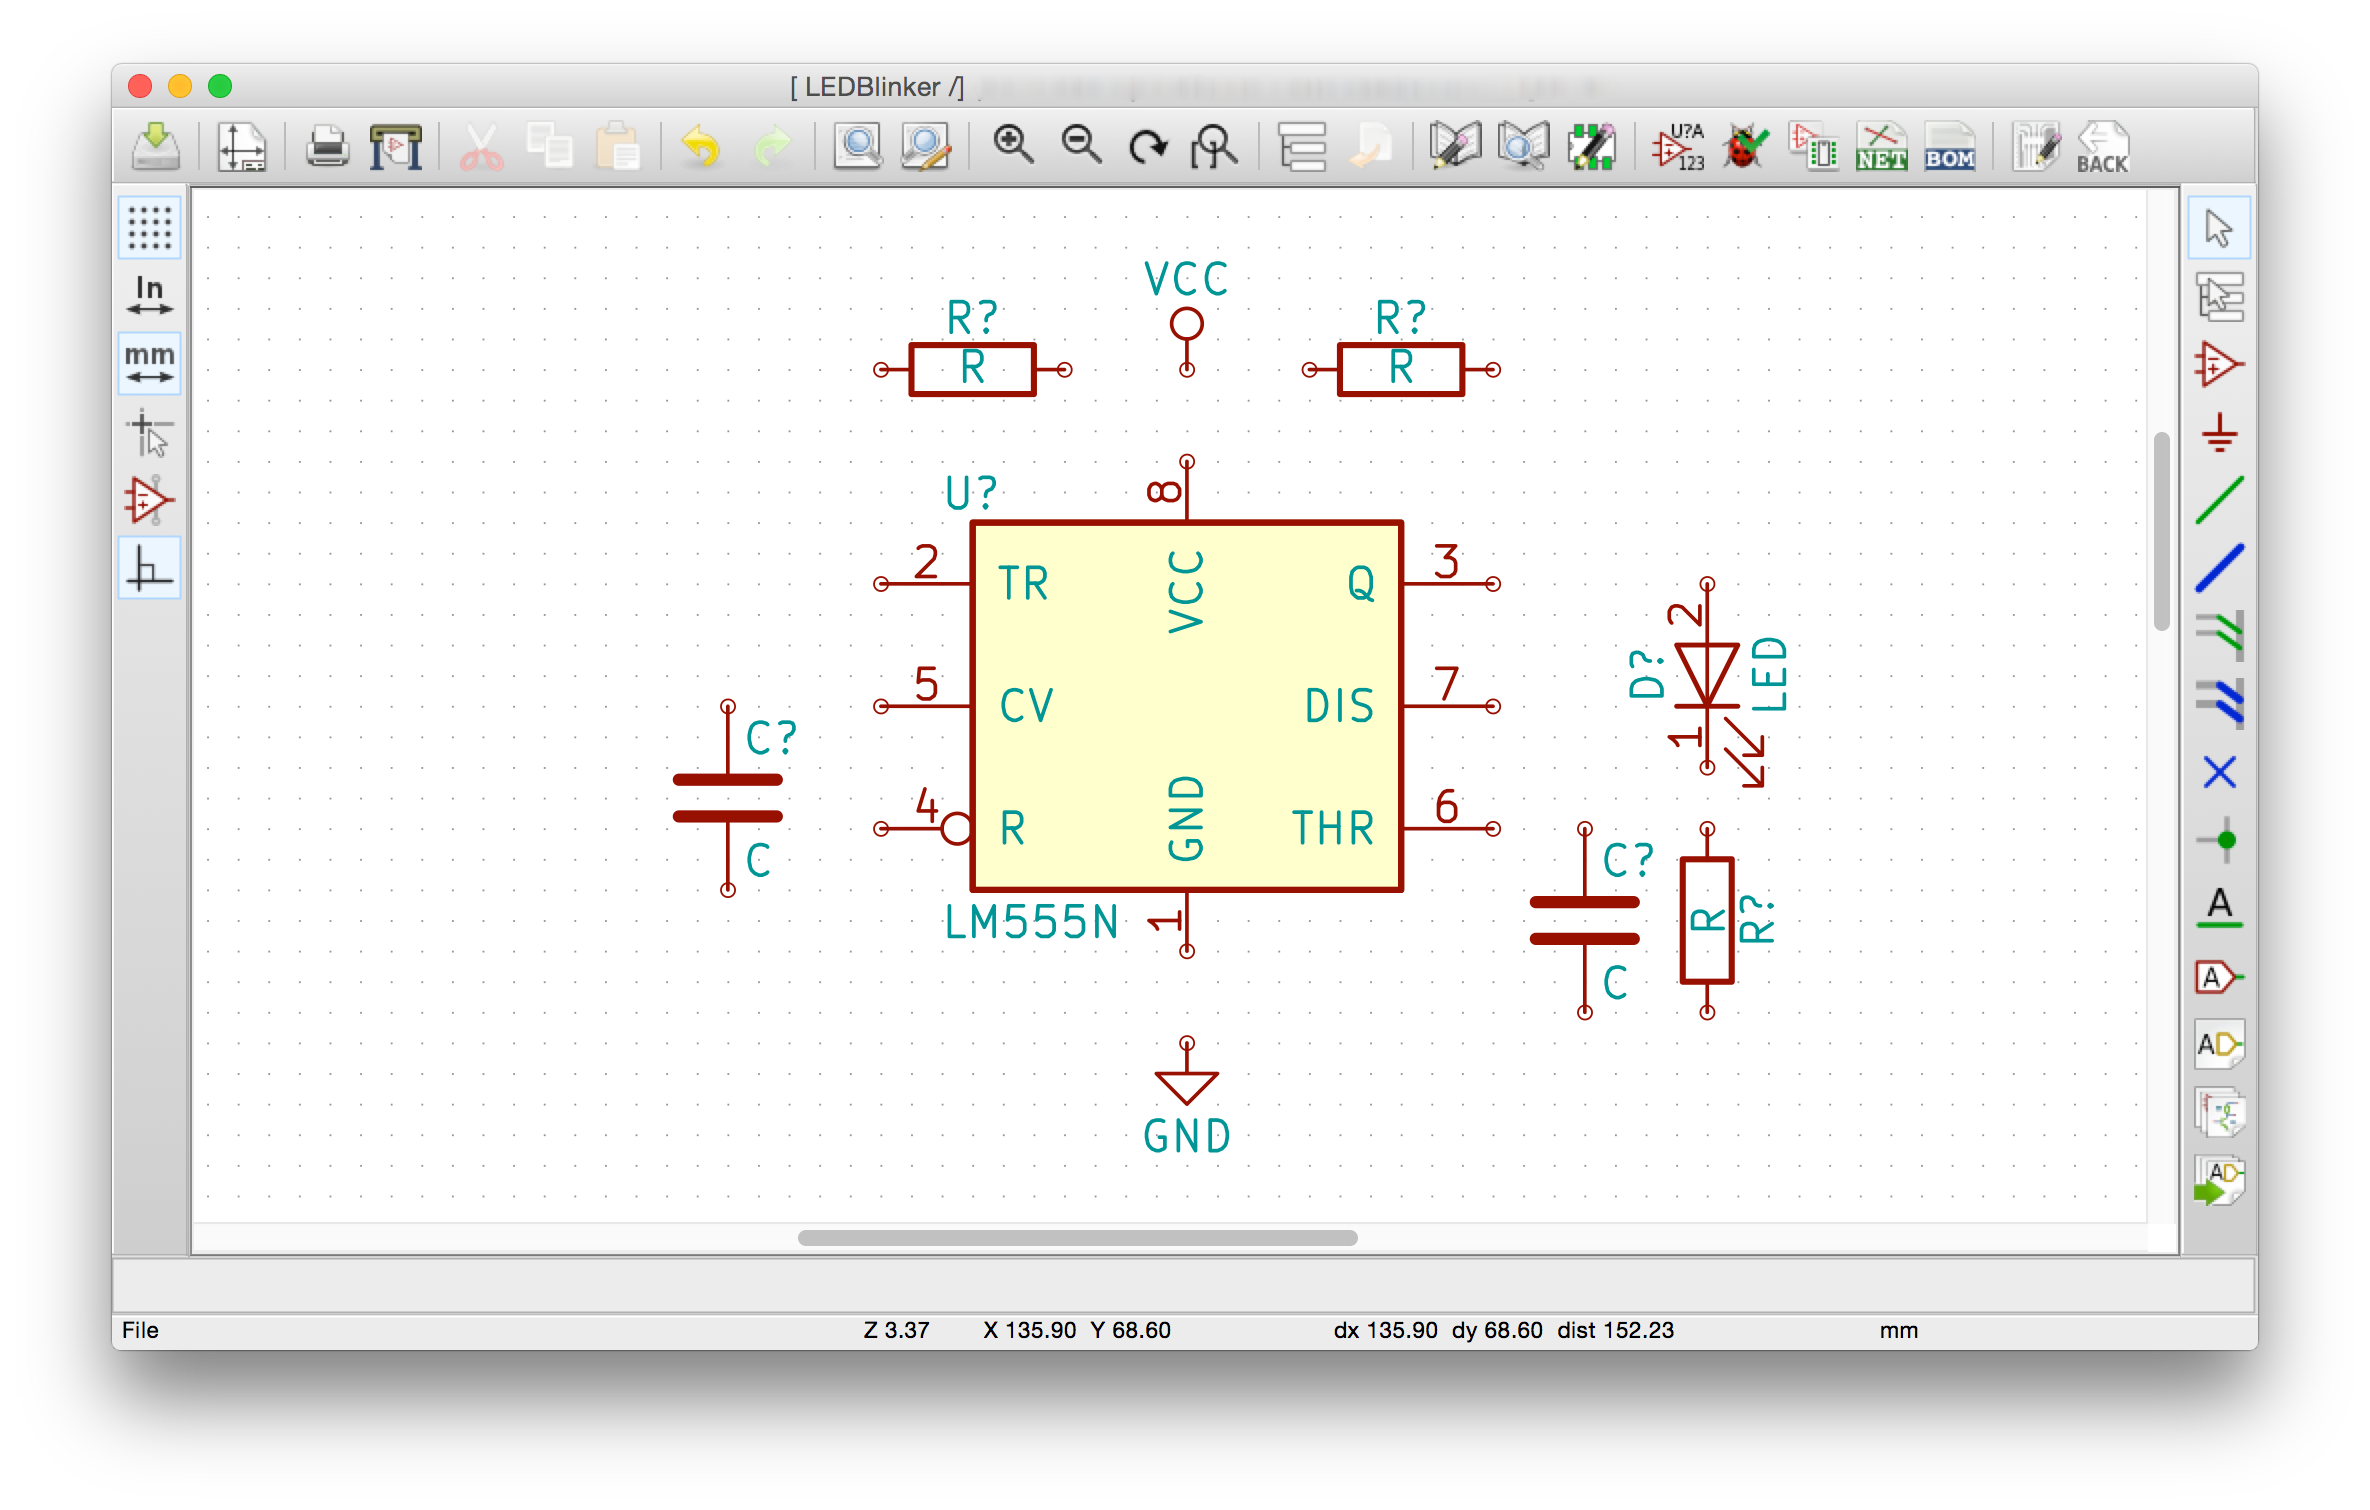
\includegraphics[width=0.75\textwidth]{RearrangedComponents}
\centering
\caption{Components Rearranged}
\end{figure}

\subsection{Adding Connections}
Now that our components in place, we need to add the connections between them. Press the button with a green line on it to select the Place Wire tool. Alternatively, the default hotkey is `\textbf{W}'.

\begin{figure}[H]

\includegraphics{PlaceWire}
\centering
\caption{Place Wire Tool}
\end{figure}

Click on the pins (the small circles) of the components to start wires, then drag over to another pin and click to make a connection. Start by connecting the ground pin (pin 1 of the LM555) to the ground power symbol and the VCC pin (pin 8 of the LM555) to the VCC power symbol. 

\begin{figure}[H]
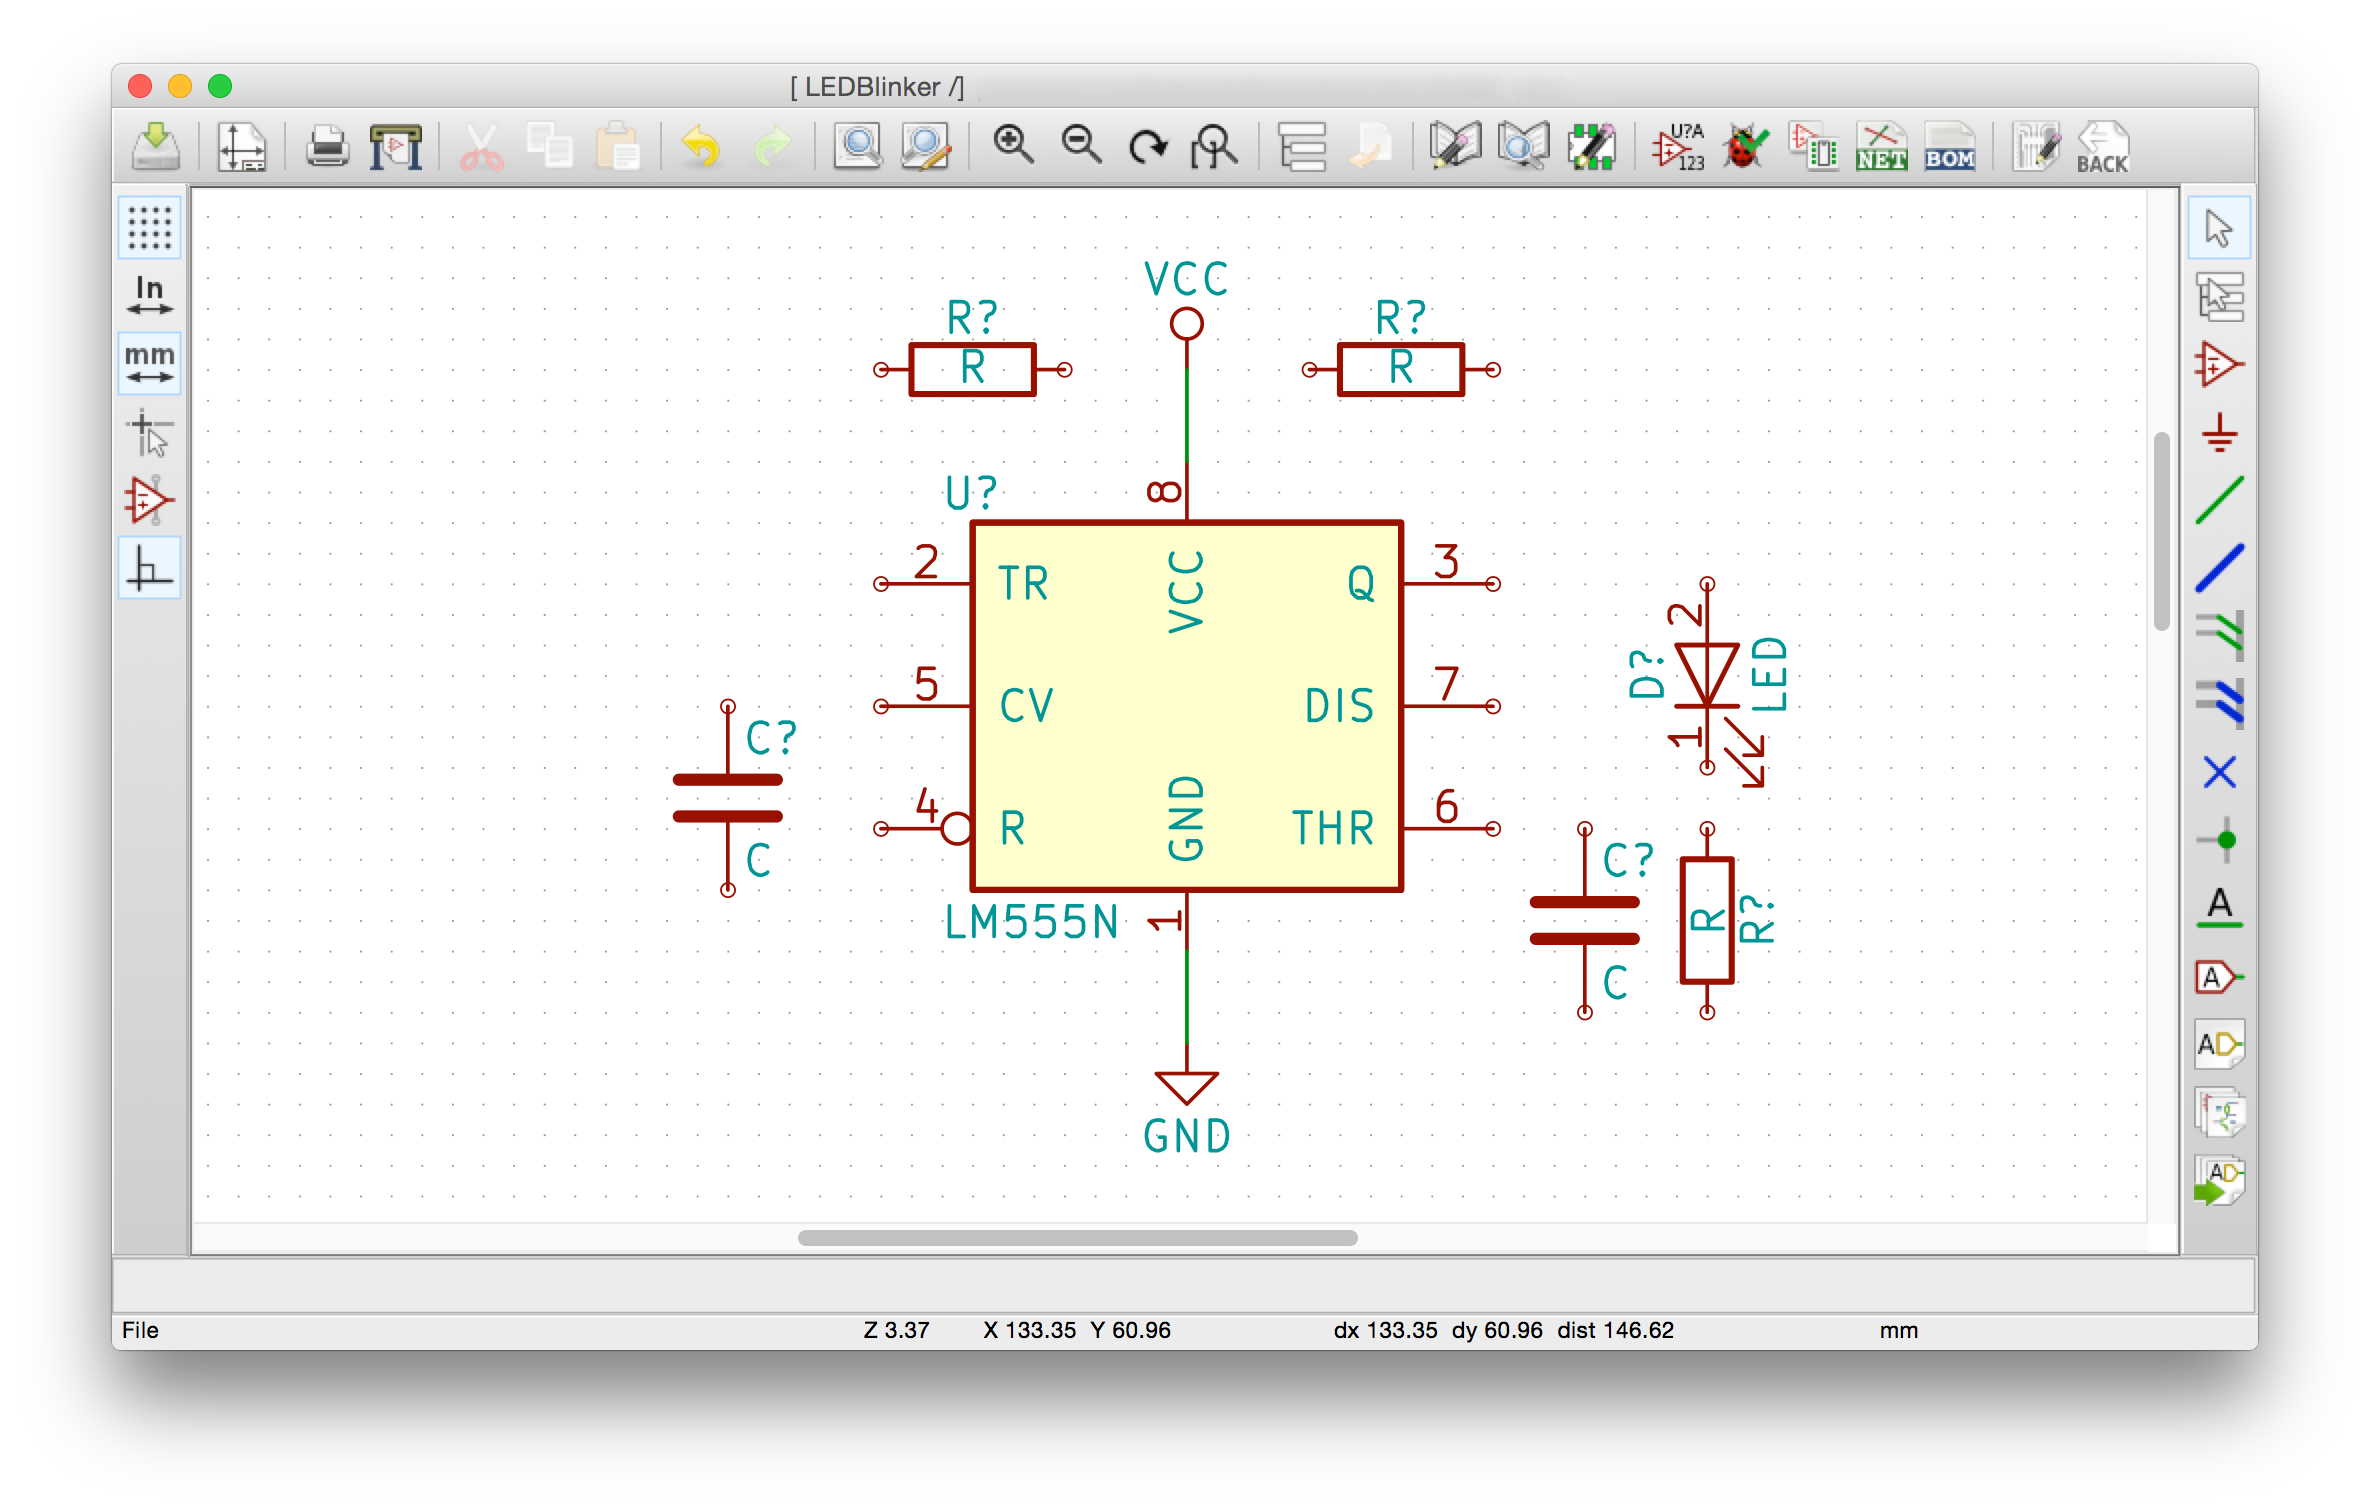
\includegraphics[width=0.75\textwidth]{ConnectPower}
\centering
\caption{Add Power Connections}
\end{figure}

Follow the example schematic to make the rest of the needed connections. If you end a wire by clicking on another wire, KiCad will automatically make a junction. Wires that cross without a junction do not connect. See the example below for reference.

If you need to move a component that already has wires connected to it, the Grab tool (default hotkey \textbf{`G'}) may be useful. This acts similarly to Move, but tries to keep existing connections. The grab tool also works on wire corners and junctions, which is useful for tidying up connections.

\begin{figure}[H]
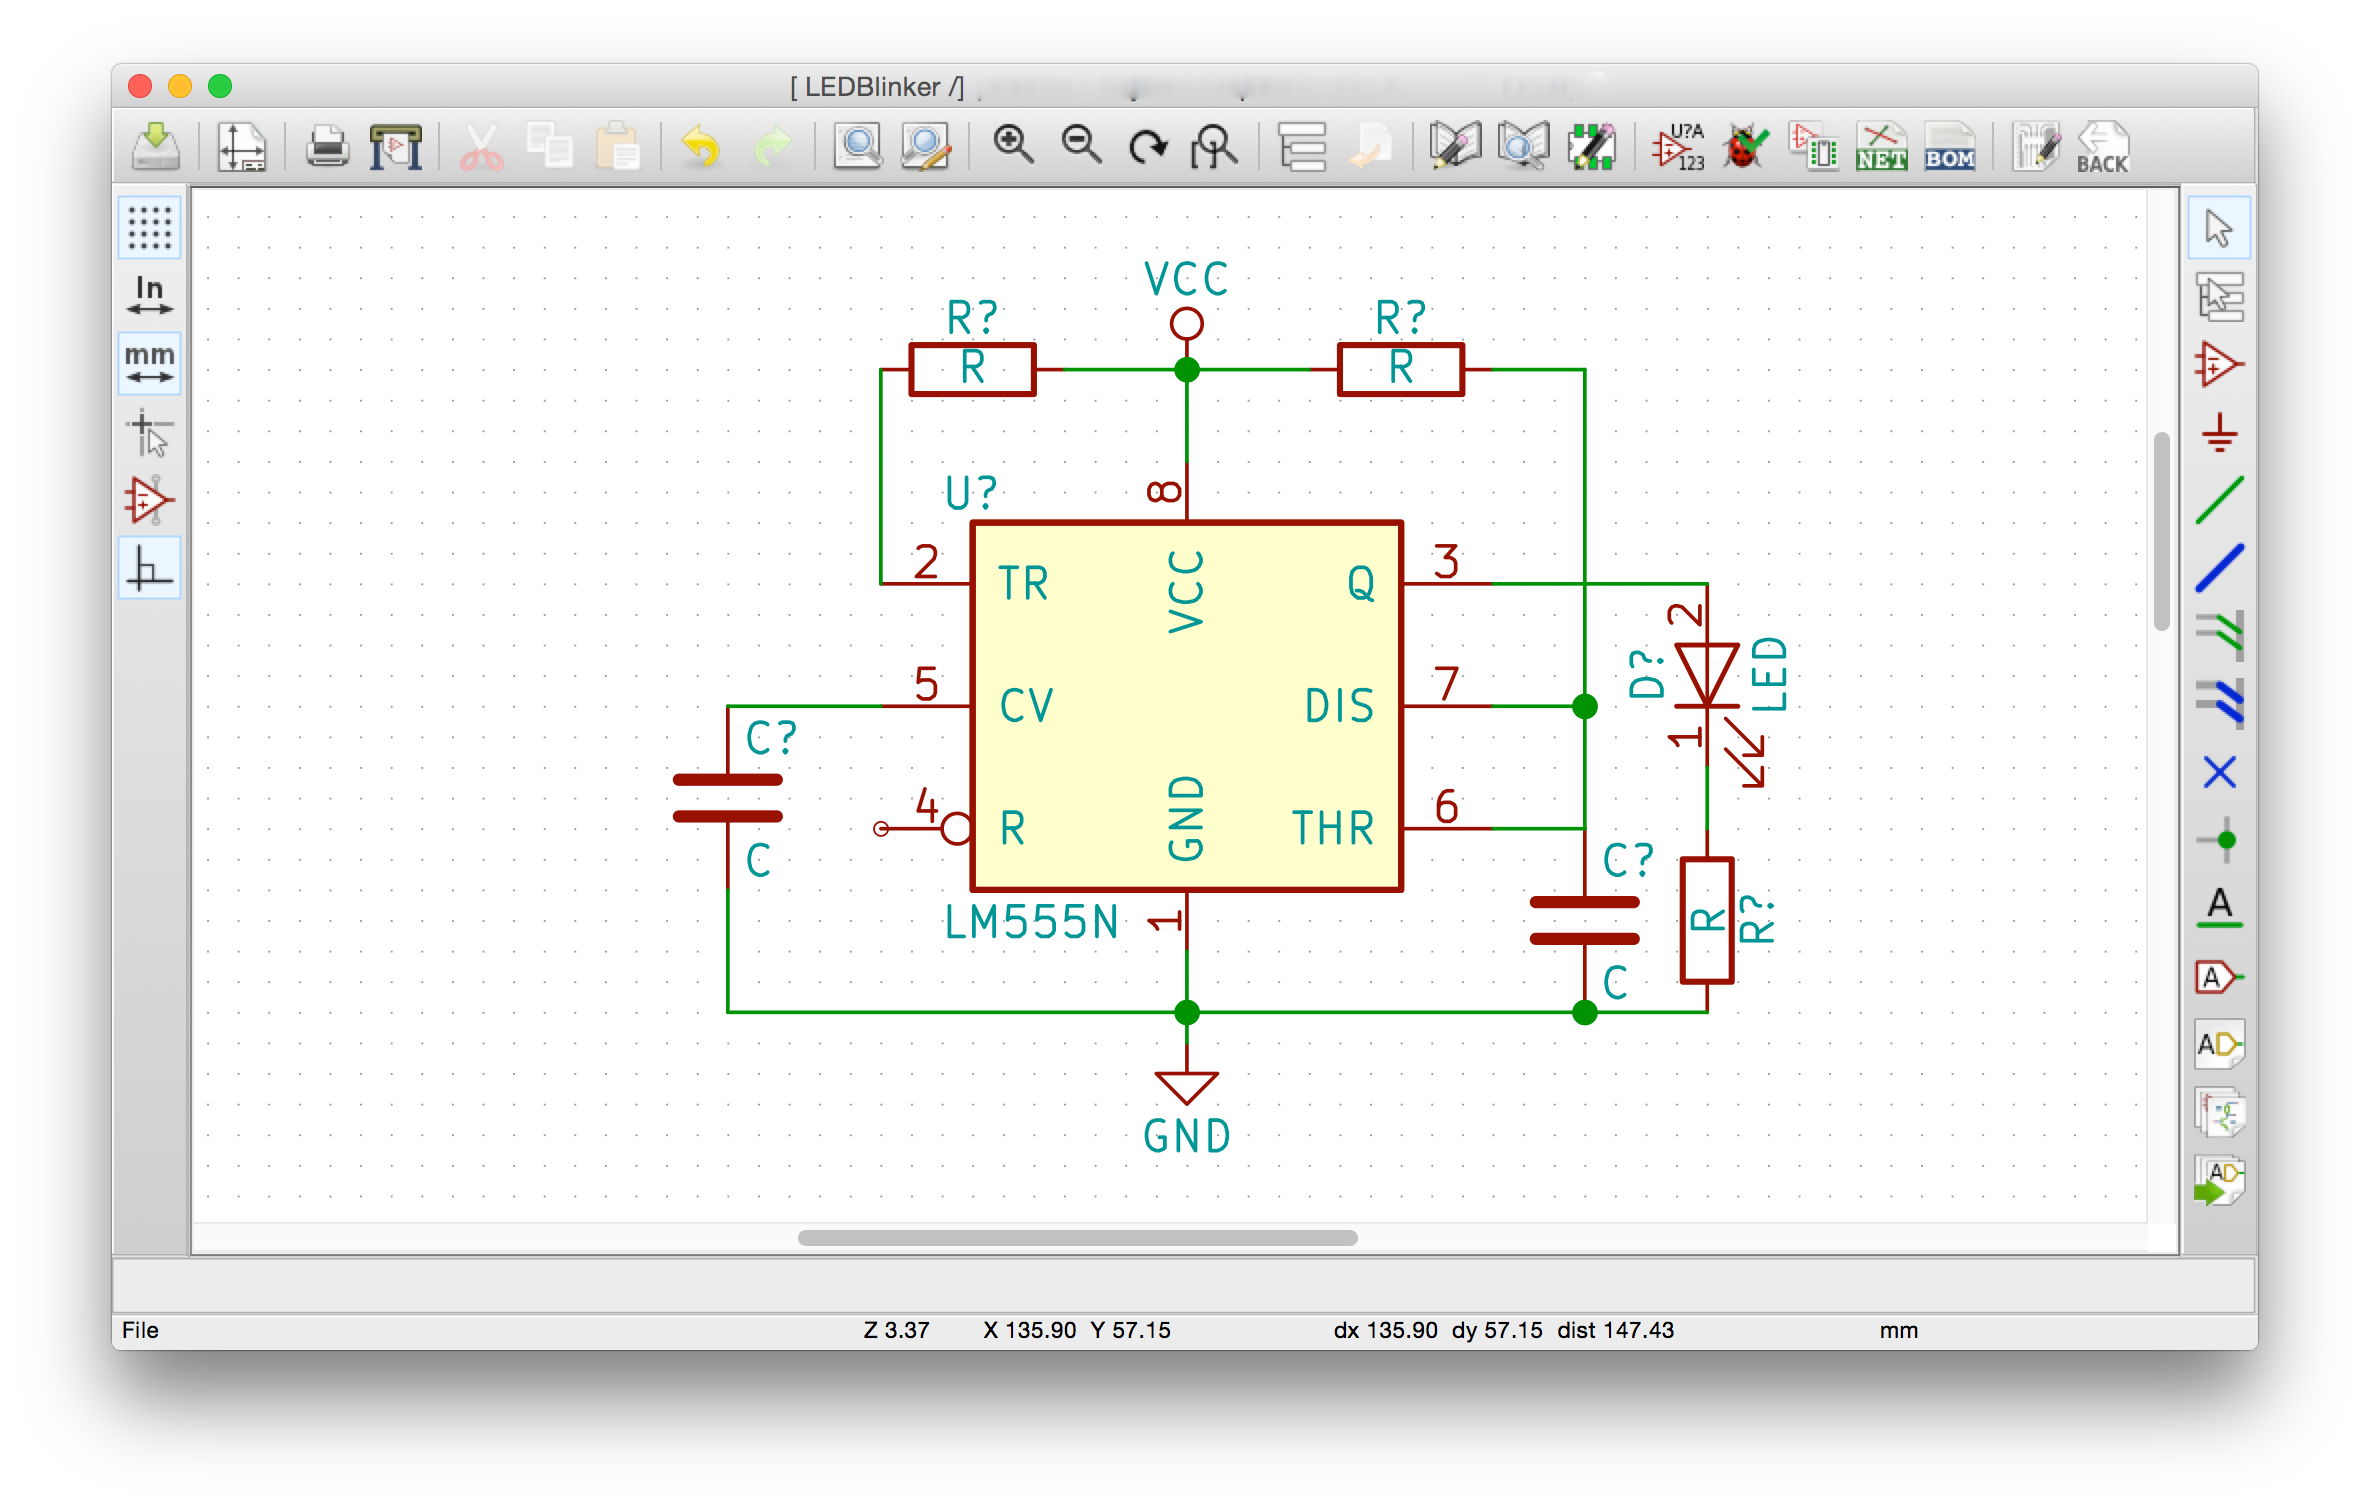
\includegraphics[width=0.75\textwidth]{SchematicConnections}
\centering
\caption{Circuit Connections Example}
\end{figure}

\subsection{Defining Values}
The components have been connected, but we still need to define the values of the passive components. Right click on one of the resistors or components and in the popup menu that appears, select \textbf{Edit Component $\rightarrow$ Value}. A dialog will appear where you can enter the appropriate value. 

\begin{figure}[H]
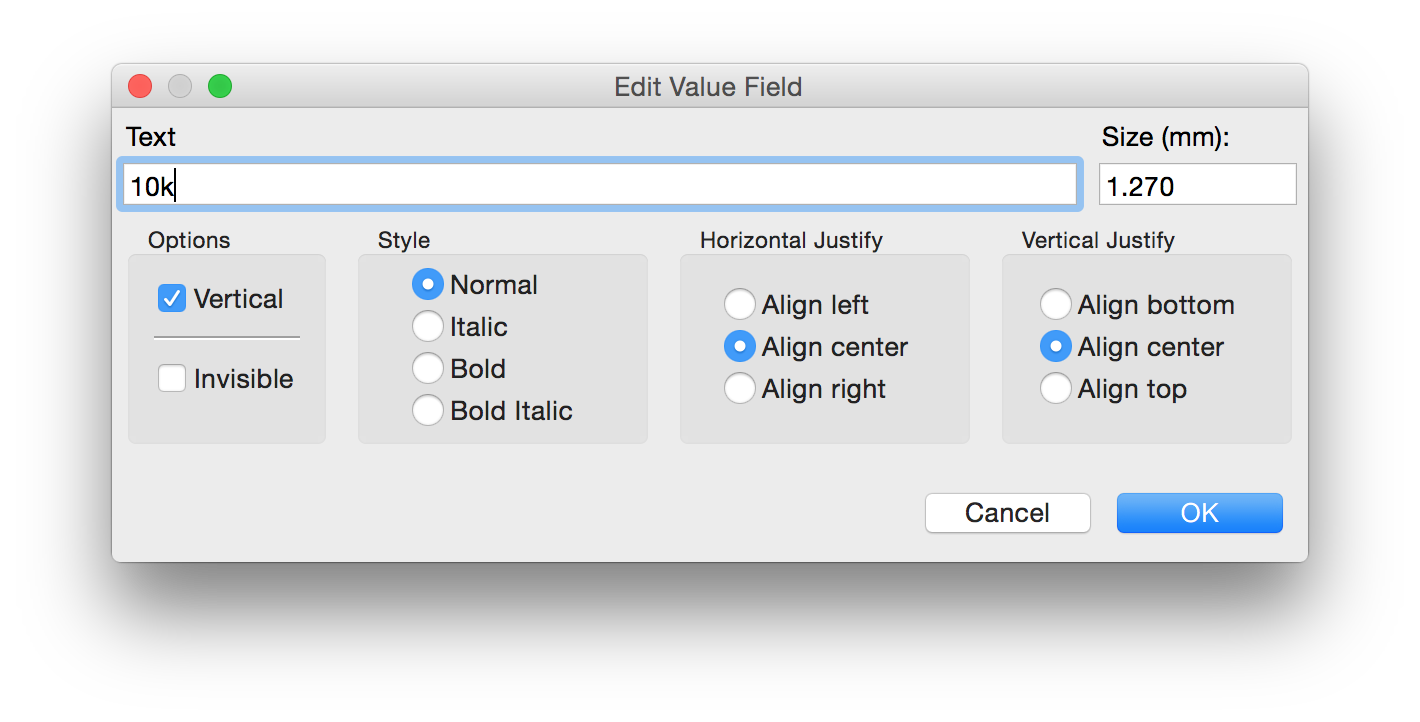
\includegraphics[width=0.75\textwidth]{EditValue}
\centering
\caption{Edit Value Dialog}
\end{figure}

When you click OK, the label on the schematic should update with the correct value. Once you've finished labeling all the resistors and capacitors, the schematic should look something like this:

\begin{figure}[H]
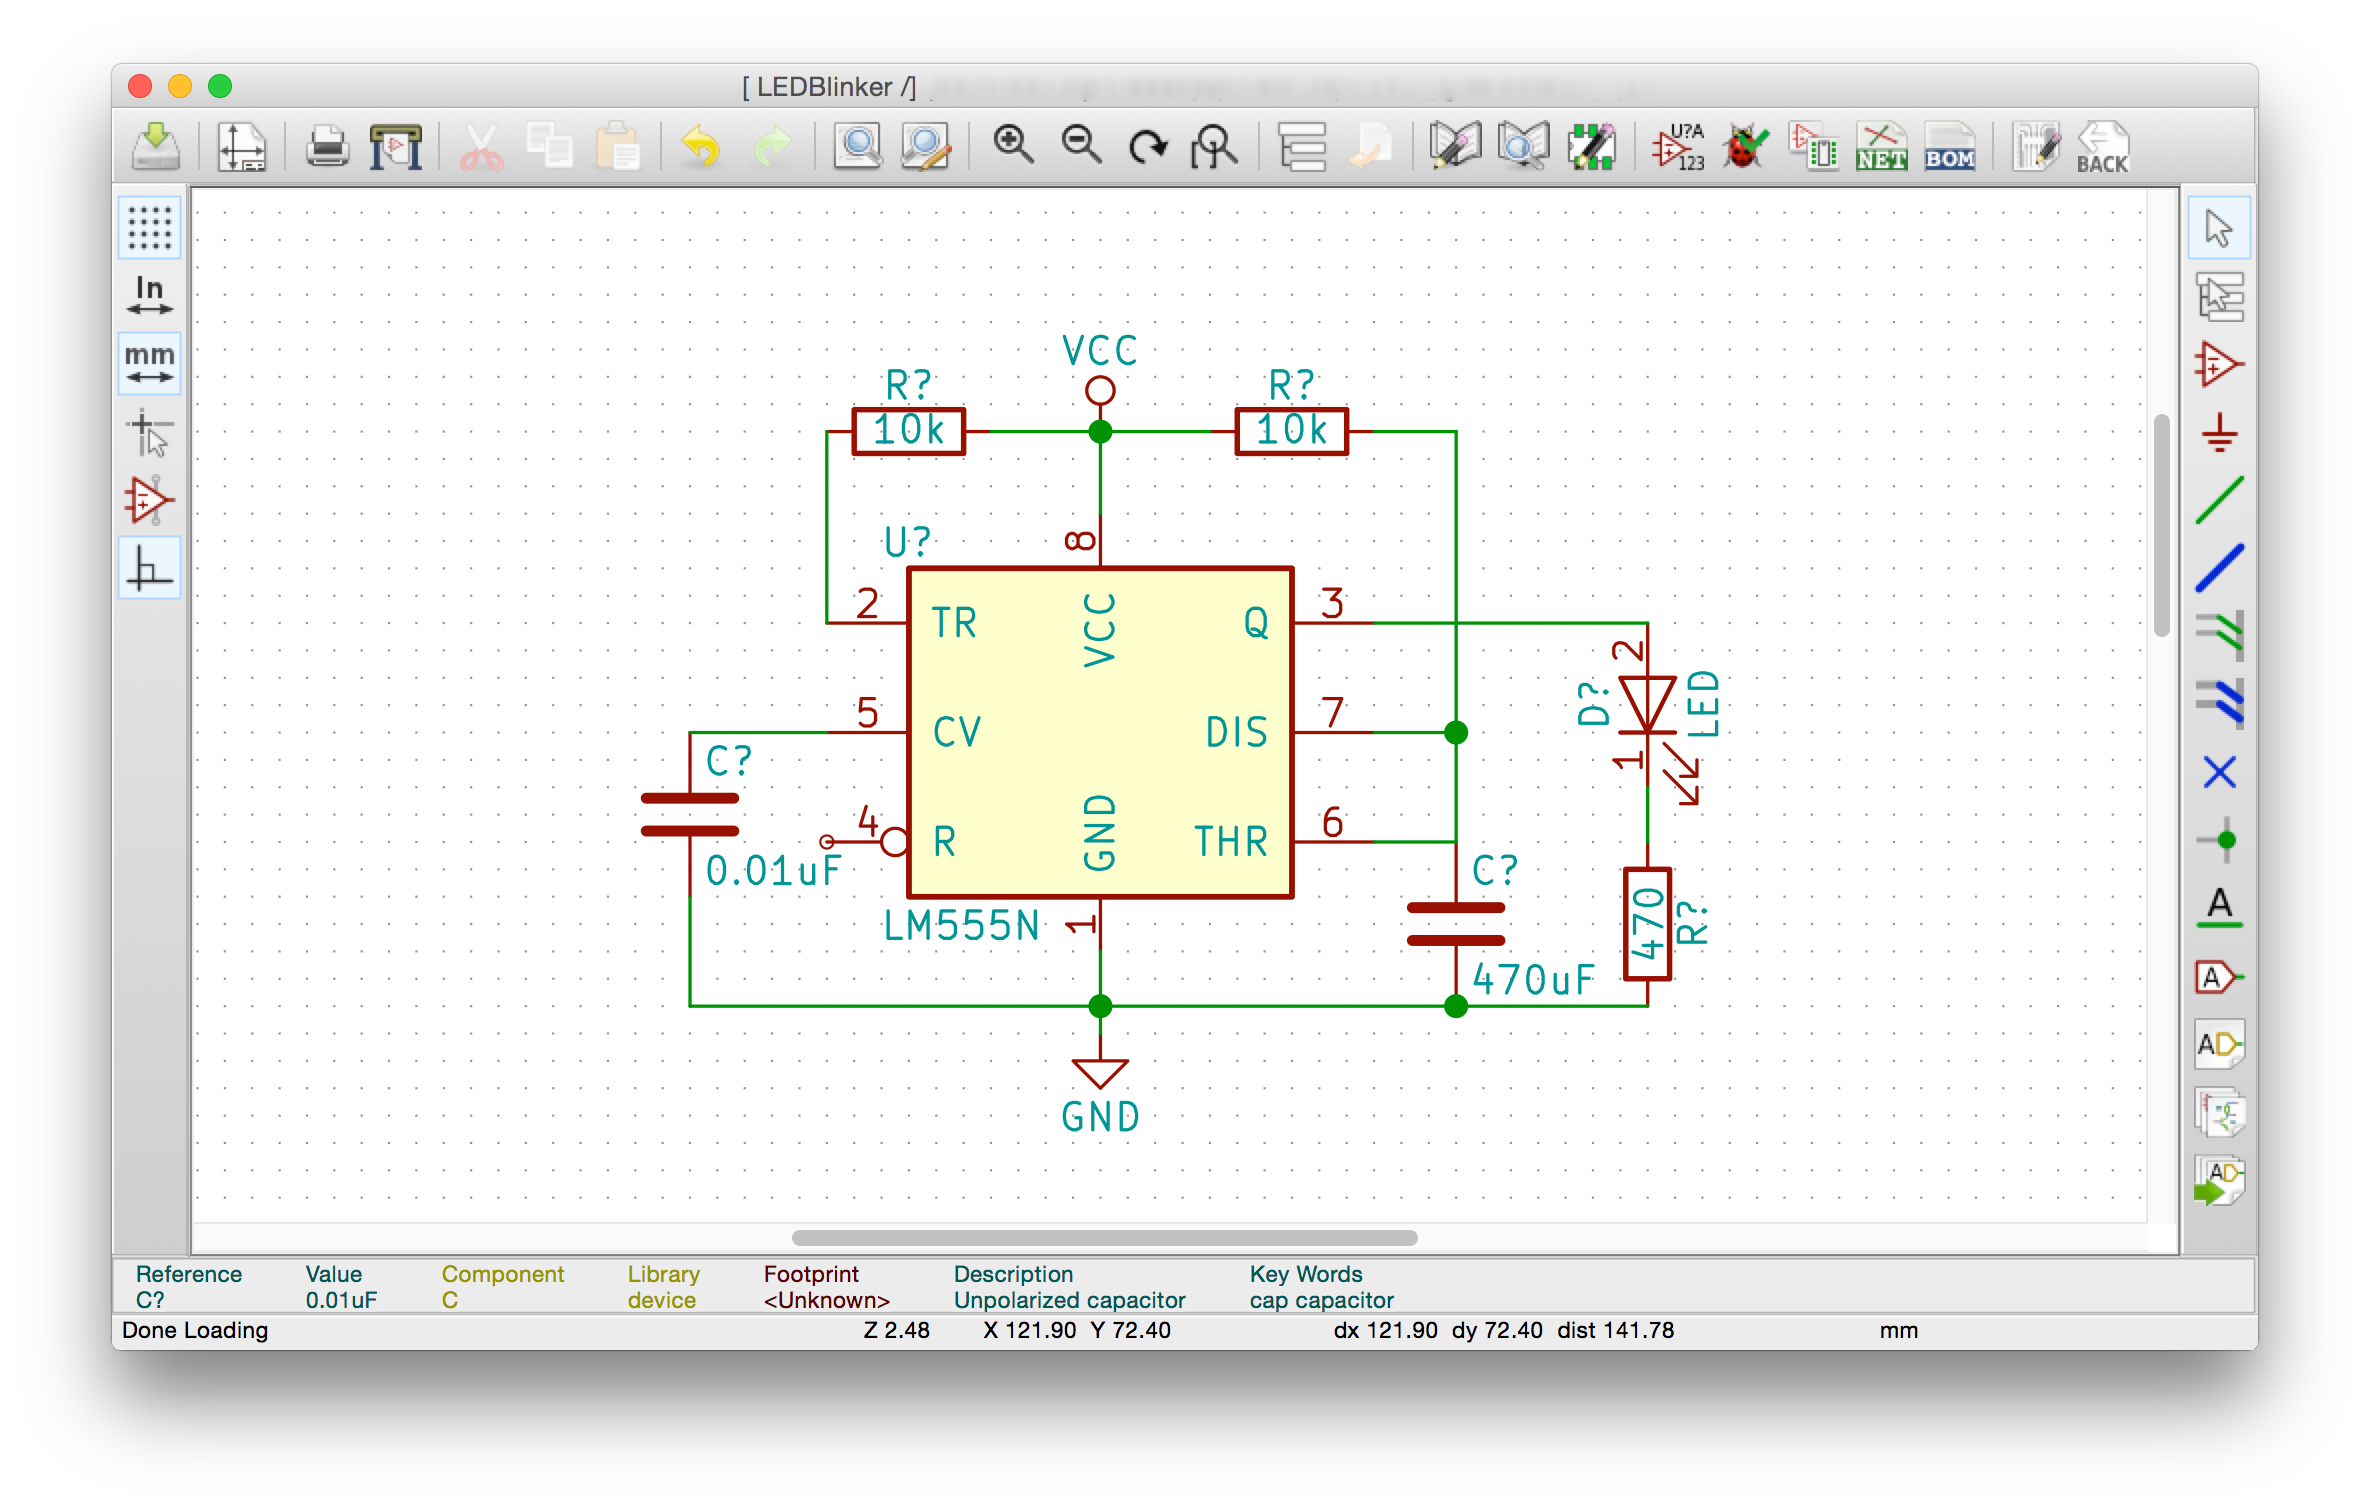
\includegraphics[width=0.75\textwidth]{AddedValues}
\centering
\caption{Schematic with Values Added}
\end{figure}

\subsection{Annotate Schematic}
Now all the information from the datasheet has been entered, and we just have a few final steps before we can start the physical layout. First, we need to give unique ID numbers to all the components. Notice that up to now, every component has had a placeholder identifier like `R?' or `C?'. On the top menu bar, locate the button labeled with an op-amp and the numbers 123.

\begin{figure}[H]

\includegraphics{AnnotateSchematicButton}
\centering
\caption{Annotate Schematic Button}
\end{figure}

When you press it, a dialog will appear showing options on how to assign the identifiers. Choose the \textbf{`Use the entire schematic'} and \textbf{`Keep existing annotation'} options, but leave the rest at their default settings.

\begin{figure}[H]
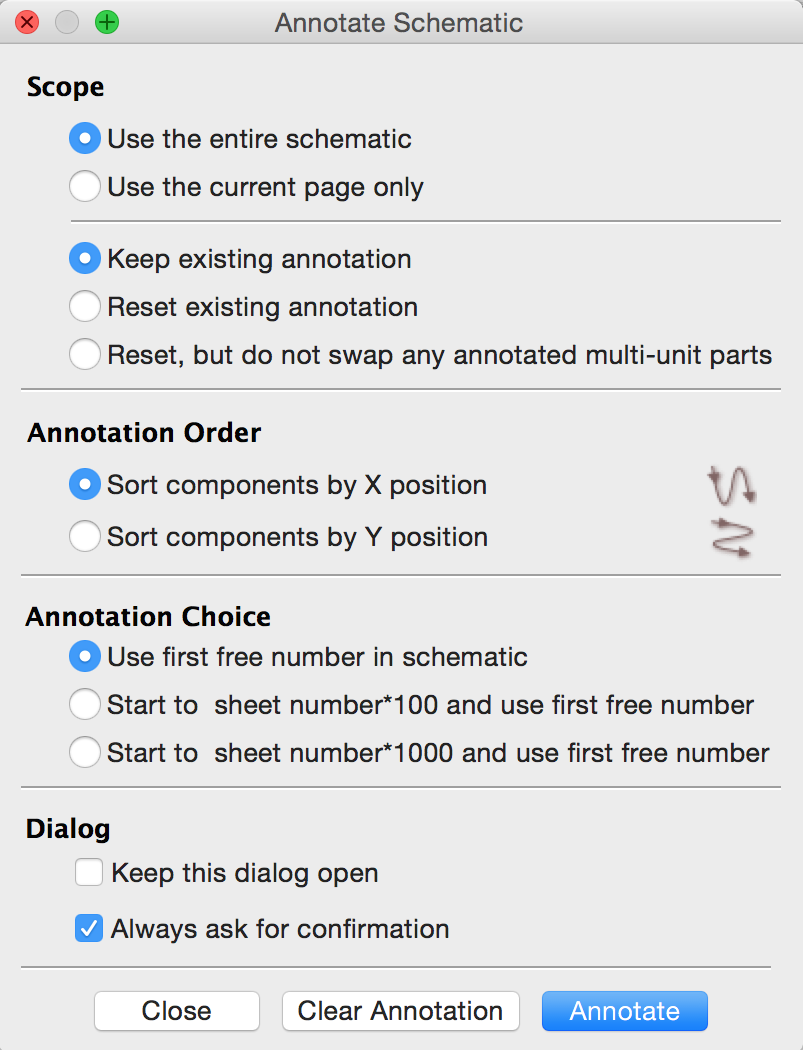
\includegraphics[width=0.5\textwidth]{AnnotateSchematic}
\centering
\caption{Annotate Schematic Dialog}
\end{figure}

Click the \textbf{Annotate} button to run the numbering utility. Now you should see that every component has a unique number assigned to it.

\begin{figure}[H]
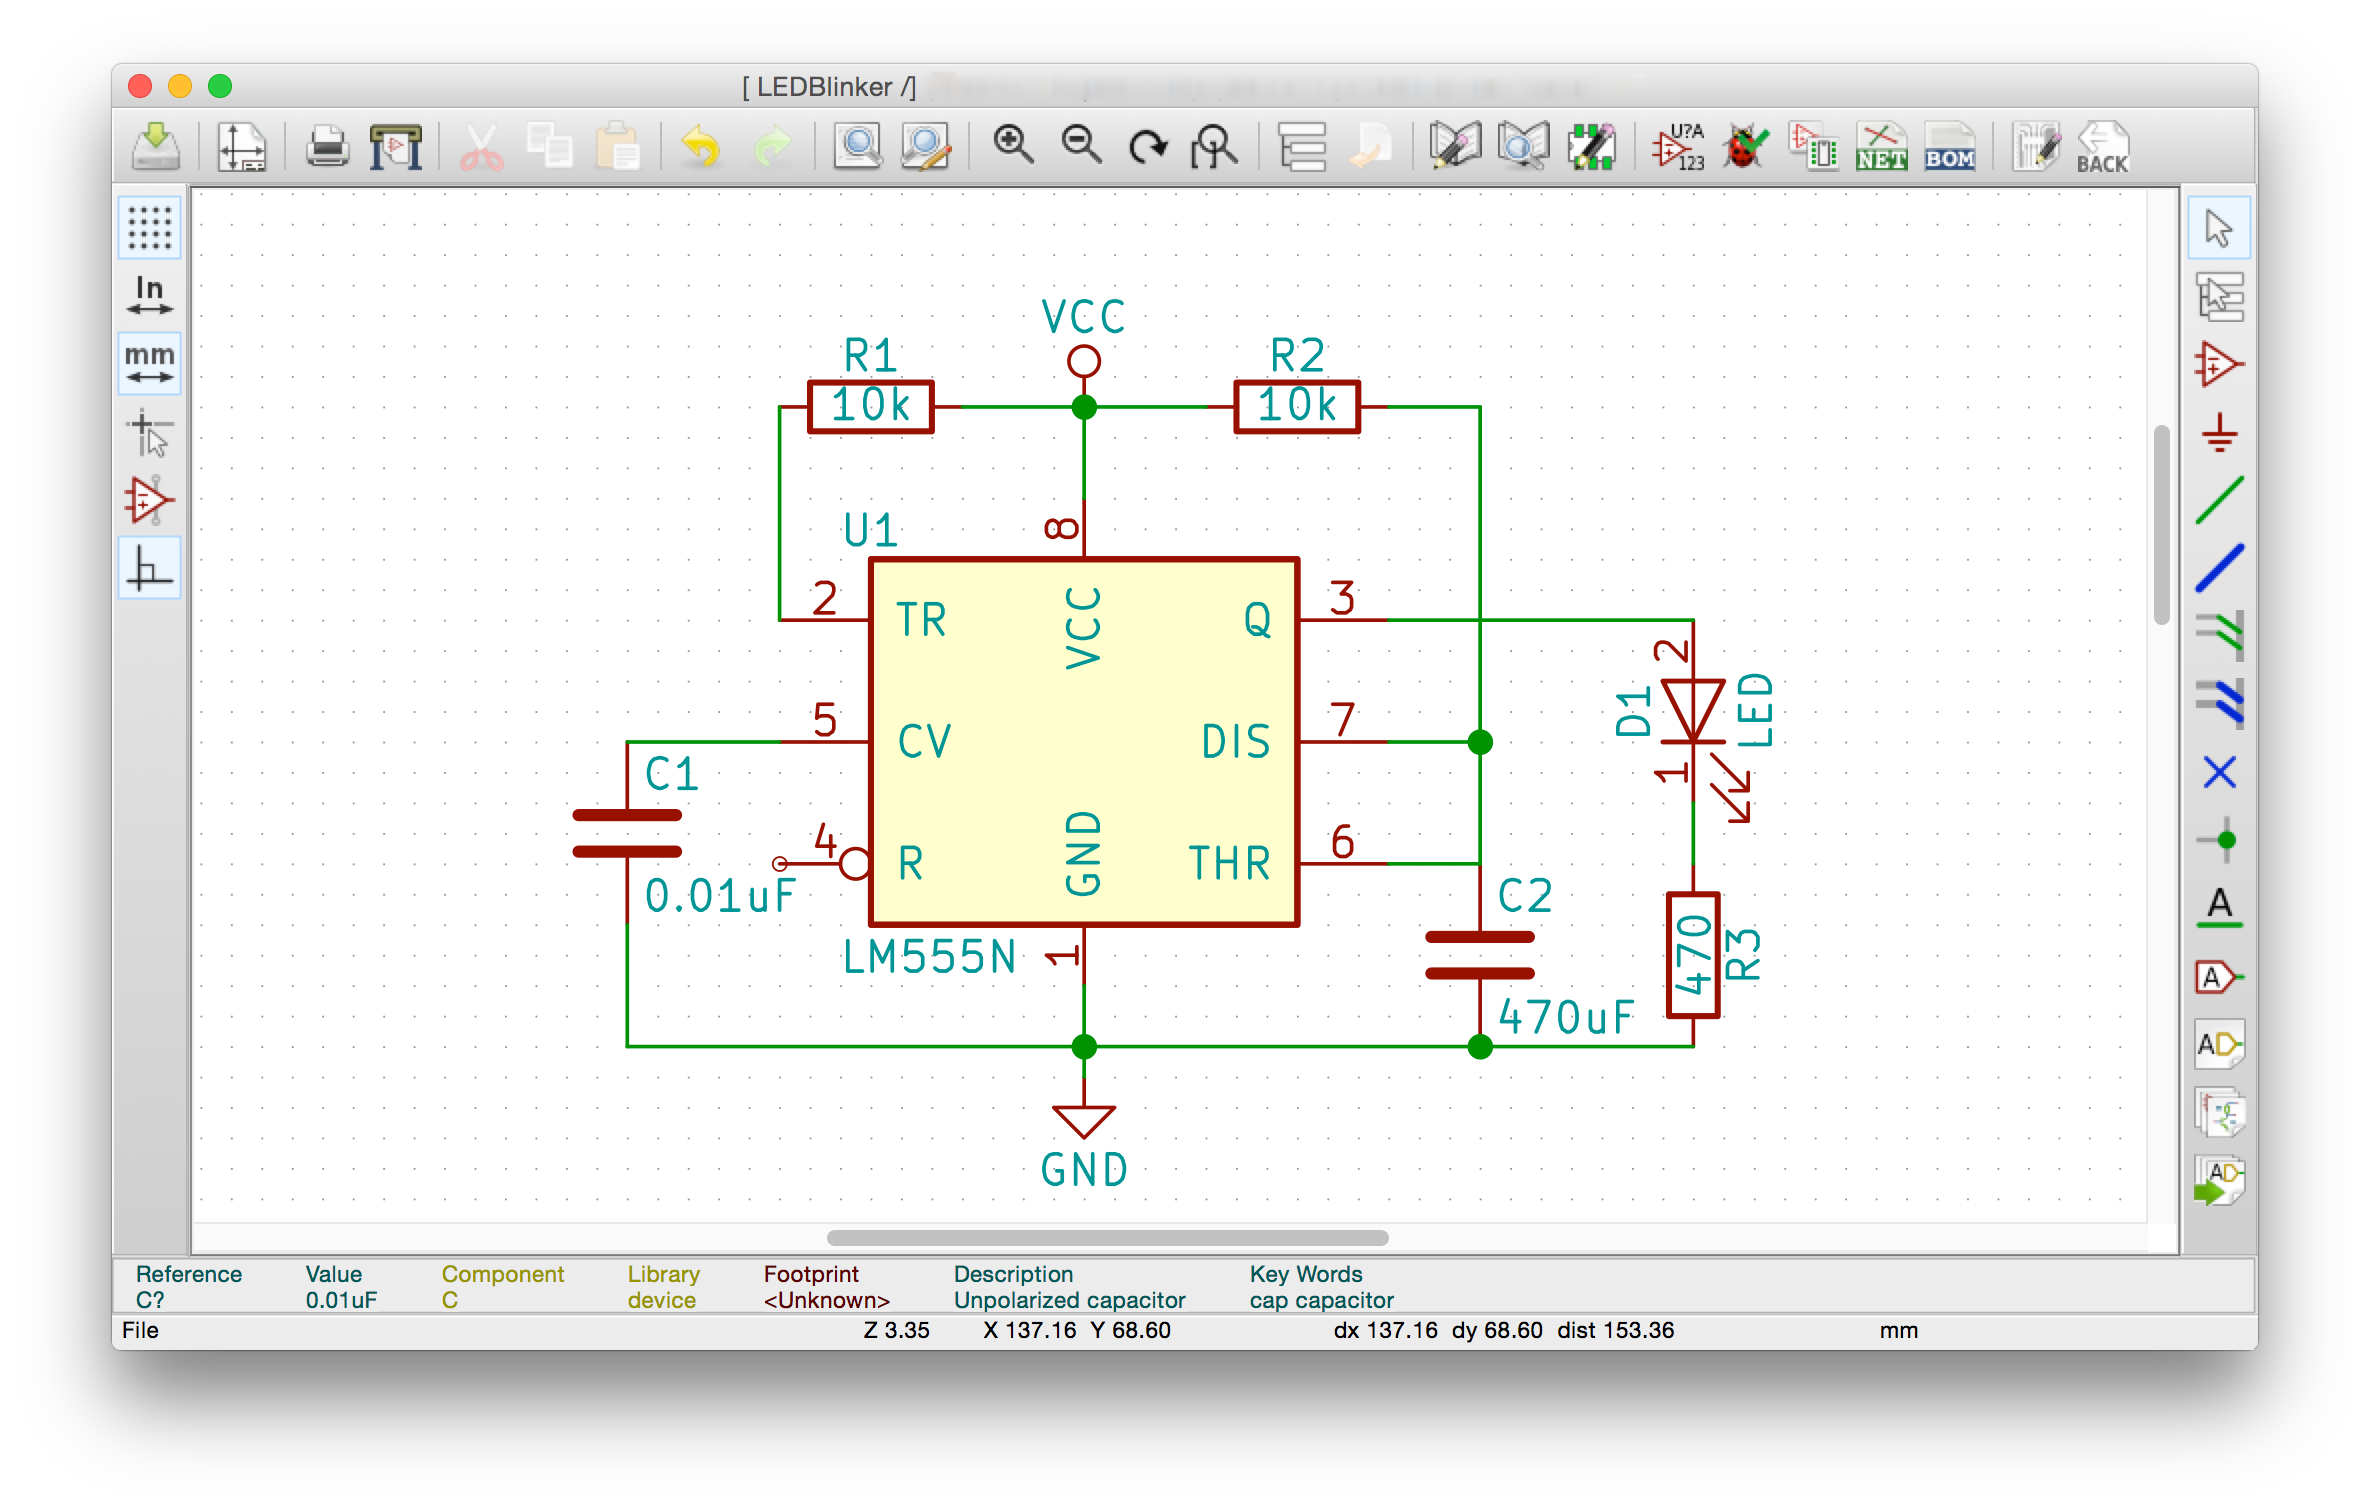
\includegraphics[width=0.75\textwidth]{SchematicAnnotated}
\centering
\caption{Annotated Schematic}
\end{figure}

\subsection{Assign Footprints}
Now we need to tell the PCB editor what footprints to use for each component. Since most components come in many different variants with different shapes and sizes, KiCad doesn't explicitly assign a footprint (physical hole/pad pattern) to each schematic symbol. Instead, you can choose a different footprint depending on what component style you have on hand or decide to order. 

Click the button two over from the annotate schematic button, with the op amp and IC shapes on it. This is the CVPcb utility for matching components to footprints.

\begin{figure}[H]

\includegraphics{CVPcbButton}
\centering
\caption{Footprint Matching Tool Button}
\end{figure}

A dialog should open up with three columns. On the left is a list of known component libraries. As you can see, footprints are organized by type of component. In the middle is a list of all the components in your schematic. On the right is a list of all the footprints within the currently selected library. 

The rightmost three buttons in the menu bar represent filtering options. Usually, I check the middle one, which filters by number of pins, and the right one, which filters by the selected library. When you have a footprint selected, the icon with a magnifying glass opens a small window that shows you what that footprint actually looks like.

\begin{figure}[H]
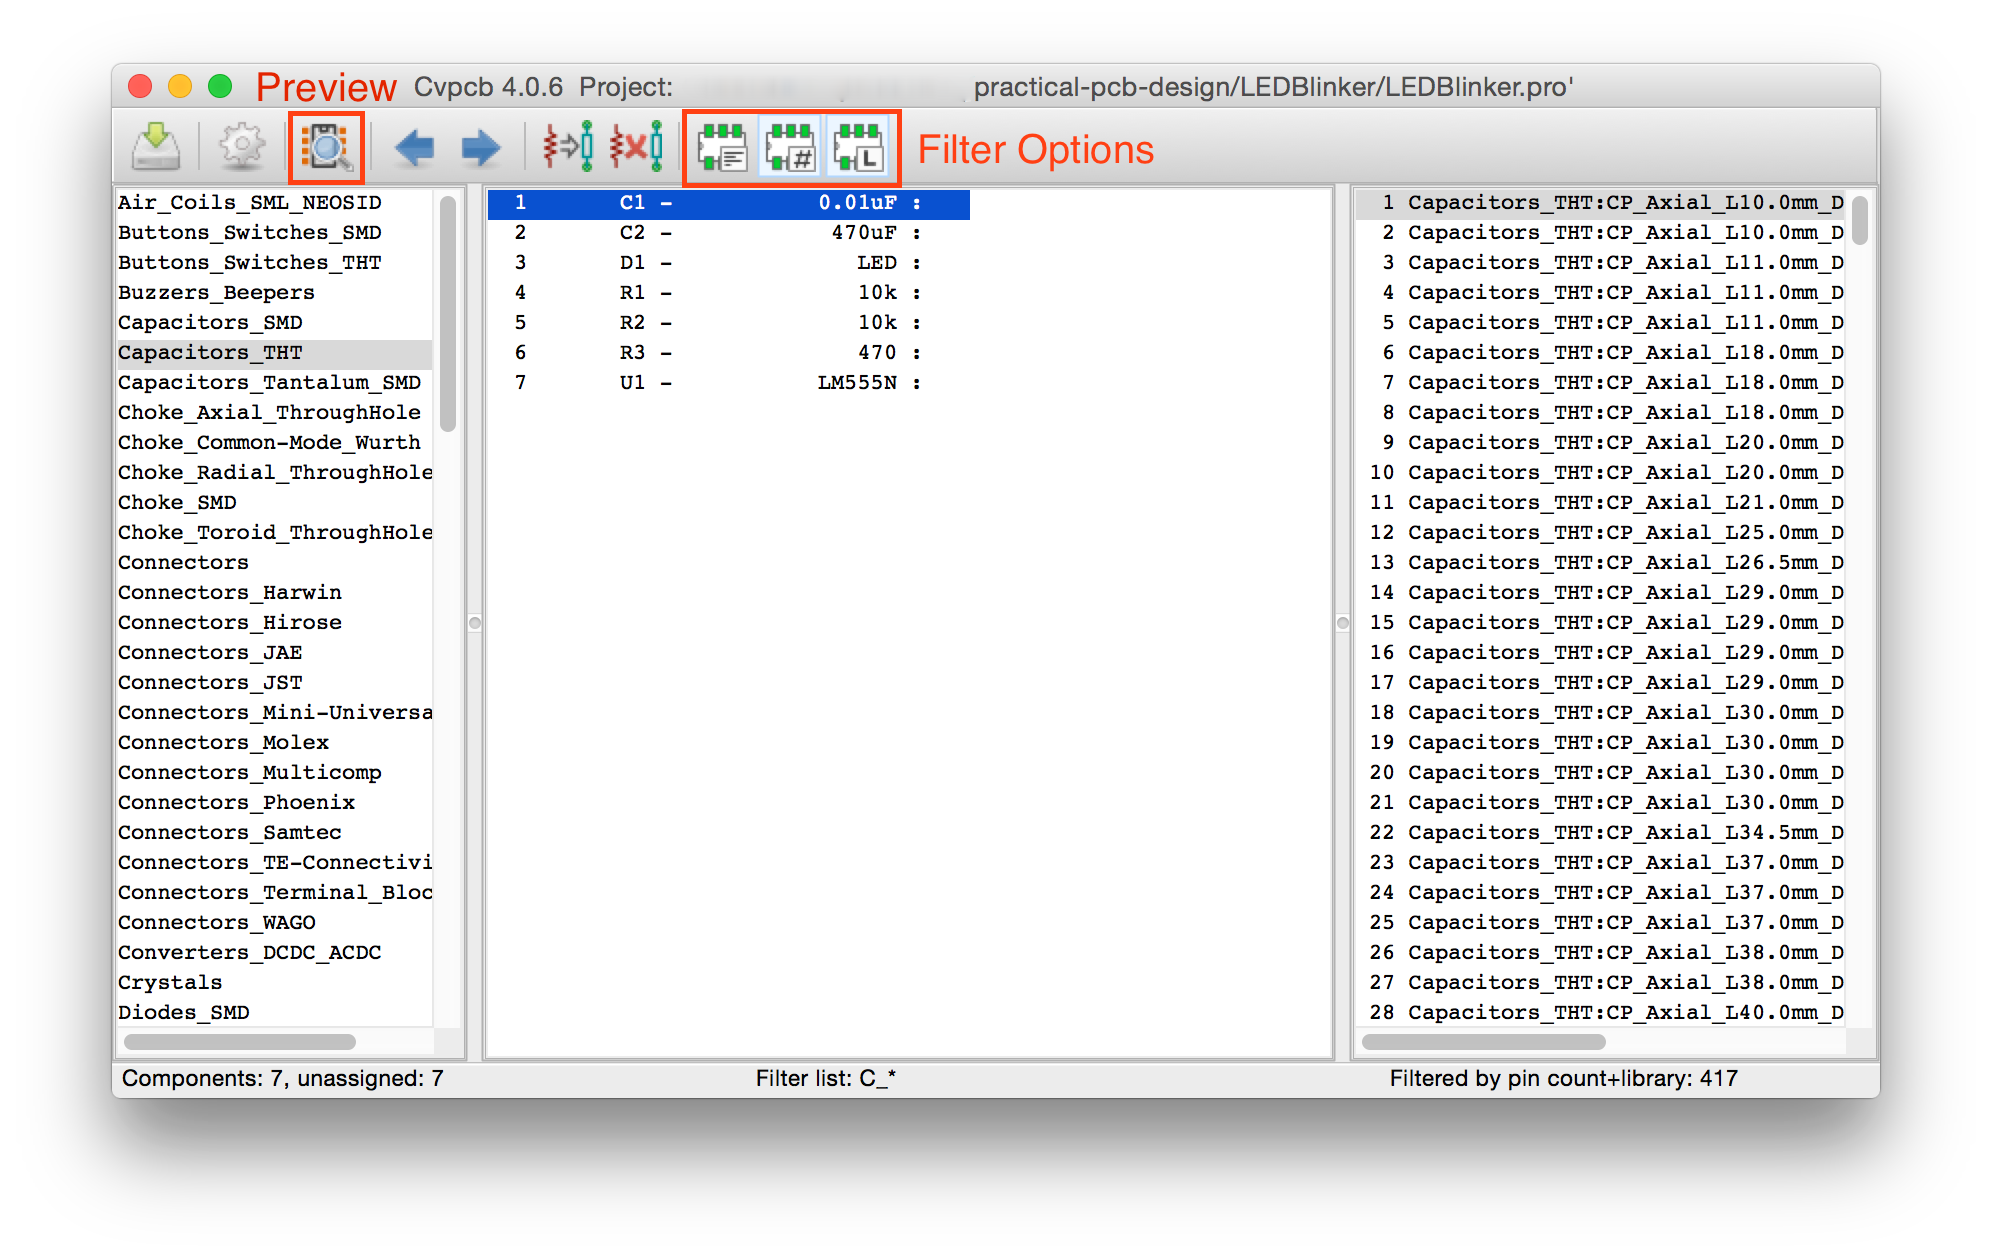
\includegraphics[width=0.75\textwidth]{CVPcb}
\centering
\caption{Selecting a Footprint}
\end{figure}

Some of the libraries or footprints are labeled with \texttt{THT}, representing Through Hole, or \texttt{SMD}, representing Surface Mount Device. These are the two most general categories of component styles. Through hole components have wire leads as connections, which are threaded through holes in the PCB and soldered. Surface mount devices are soldered directly onto flat pads on one side of the PCB and tend to be much smaller than through hole components.

Click on the first component in the list, likely a capacitor. Then select the \texttt{Capacitors\_THT} library on the left, and double click one of the footprints on the right to select it. 

Assign footprints for each of your components. In practice, which footprint you select will depend on the dimensions and style of the actual component you will be using, but for this workshop I would recommend these footprints: 

\begin{tabular}{|c|c|c|}
\hline 
\textbf{Component} & \textbf{Library} & \textbf{Footprint Name} \\ 
\hline 
Capacitor & \texttt{Capacitors\_THT} & \texttt{Capacitors\_THT:C\_Radial\_D5\_L6\_P2.5} \\ 
\hline 
Resistor & \texttt{Resistors\_THT} & \texttt{Resistors\_THT:Resistor\_Horizontal\_RM7mm} \\ 
\hline 
LED & \texttt{LEDs} & \texttt{LEDs:LED-5MM} \\ 
\hline 
LM555 & \texttt{Housings\_DIP} & \texttt{Housings\_DIP:DIP-8\_W7.62mm\_Socket} \\ 
\hline 
\end{tabular}

When all the footprints have been assigned, save and close out of the dialog.

\subsection{Generate Netlist}
Now we have specified all the information we will need in the PCB editor. Click on the button labeled NET to generate the netlist.

\begin{figure}[H]

\includegraphics{NetlistButton}
\centering
\caption{Generate Netlist Button}
\end{figure}

This netlist file contains the schematic specifications in a compact format that the PCB editor can understand. Make sure PCBNew is the format selected, and hit the Generate button. Save the netlist in the same directory as the rest of the project.

\begin{figure}[H]
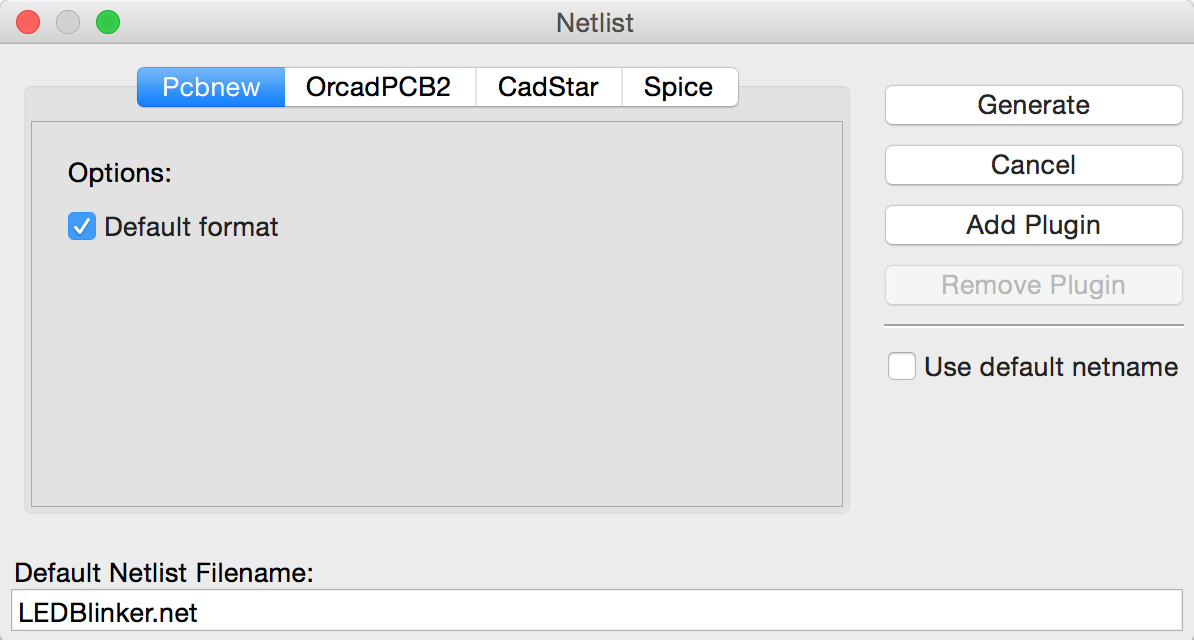
\includegraphics[width=0.5\textwidth]{NetlistDialog}
\centering
\caption{Generate Netlist Dialog}
\end{figure}

We are done with our schematic! Save and close out of the schematic editor.

\section{PCB Layout}
\subsection{Design Rules}
\subsection{Component Placement}
\subsection{Board Outline}
\subsection{Routing}
\subsection{Pours}
\subsection{Export}
\subsection{Tips and Tricks}

\section{Extra: Creating New Components}
\subsection{Schematic Symbol}

\subsection{PCB Footprint}

\end{document}